\chapter{Experimental Program}
\label{chap-three}

Corrosion is the main aging condition that affects structures. Therefore, the success of this study relies on the most accurate representation of the corrosion process in the analytical model. As mentioned in Chapter 2, previous studies developed accelerated corrosion rebar specimens with high current densities, but did not account for the depassivation process of the reinforcing steel. A main objective of this study was to verify the mechanical properties of corroded rebars while considering the depassivation process. The experimental process was divided into the following main components: (1) corroded specimens preparation, (2) tension tests on corroded rebars, (3) buckled bar tension (BBT) tests on corroded rebars, (4) 3D scans of corroded rebars, (5) SEM observations of fracture surfaces from BBT tests, and (6) tension and BBT tests on turned down corroded rebars. The results obtained from the tension and BBT tests were used  in the analytical model presented in Chapter 5, and more broadly provide accurate mechanical properties of corroded rebars.

\section{Specimen Preparation}

Rebars embedded in concrete generate a protective film that protects the rebars against corrosion, due to the alkaline environment of the cement paste. The most common form of corrosion occurs via chloride attacks. During a chloride attack, the chloride diffuses in the concrete cover and comes into contact with the surface of the rebars. This initiates the process of depassivation,    in which the protective film on the surface of the rebar is eliminated. The depassivation of the rebar enables the process of corrosion to occur. The proposed experimental campaign described in this chapter aims to simulate the process of corrosion as it would occur in rebars embedded   in concrete. Using as received rebars, that is, no special treatment to the surface of the rebar, the specimen preparation procedure consists of (1) protecting the rebar ends that will be used as grips during the tension and buckled bar tension (BBT) tests, (2) generating the passive layer on the rebars, and (3) performing accelerated corrosion of the rebars until the specified levels of corrosion.

\subsection{Preparation of Rebar Ends}

First, it was necessary to protect the areas of the rebar that functioned as grips during the tension and BBT tests against corrosion, to prevent a failure inside the grips. Therefore, the ends of the rebars were protected with three layers. The first layer consisted of two-part epoxy, the second layer consisted of electroplater tape, and the third layer consisted of shrink tube. These layers ensured minimal corrosion in the grip areas of the rebar. \fref{fig:RebarSpecimenGeomtry} and \fref{fig:RebarEndsProtection} show the specimen geometry and the protective layers at the ends of the rebars.
\begin{figure}[htbp]
	\centering
	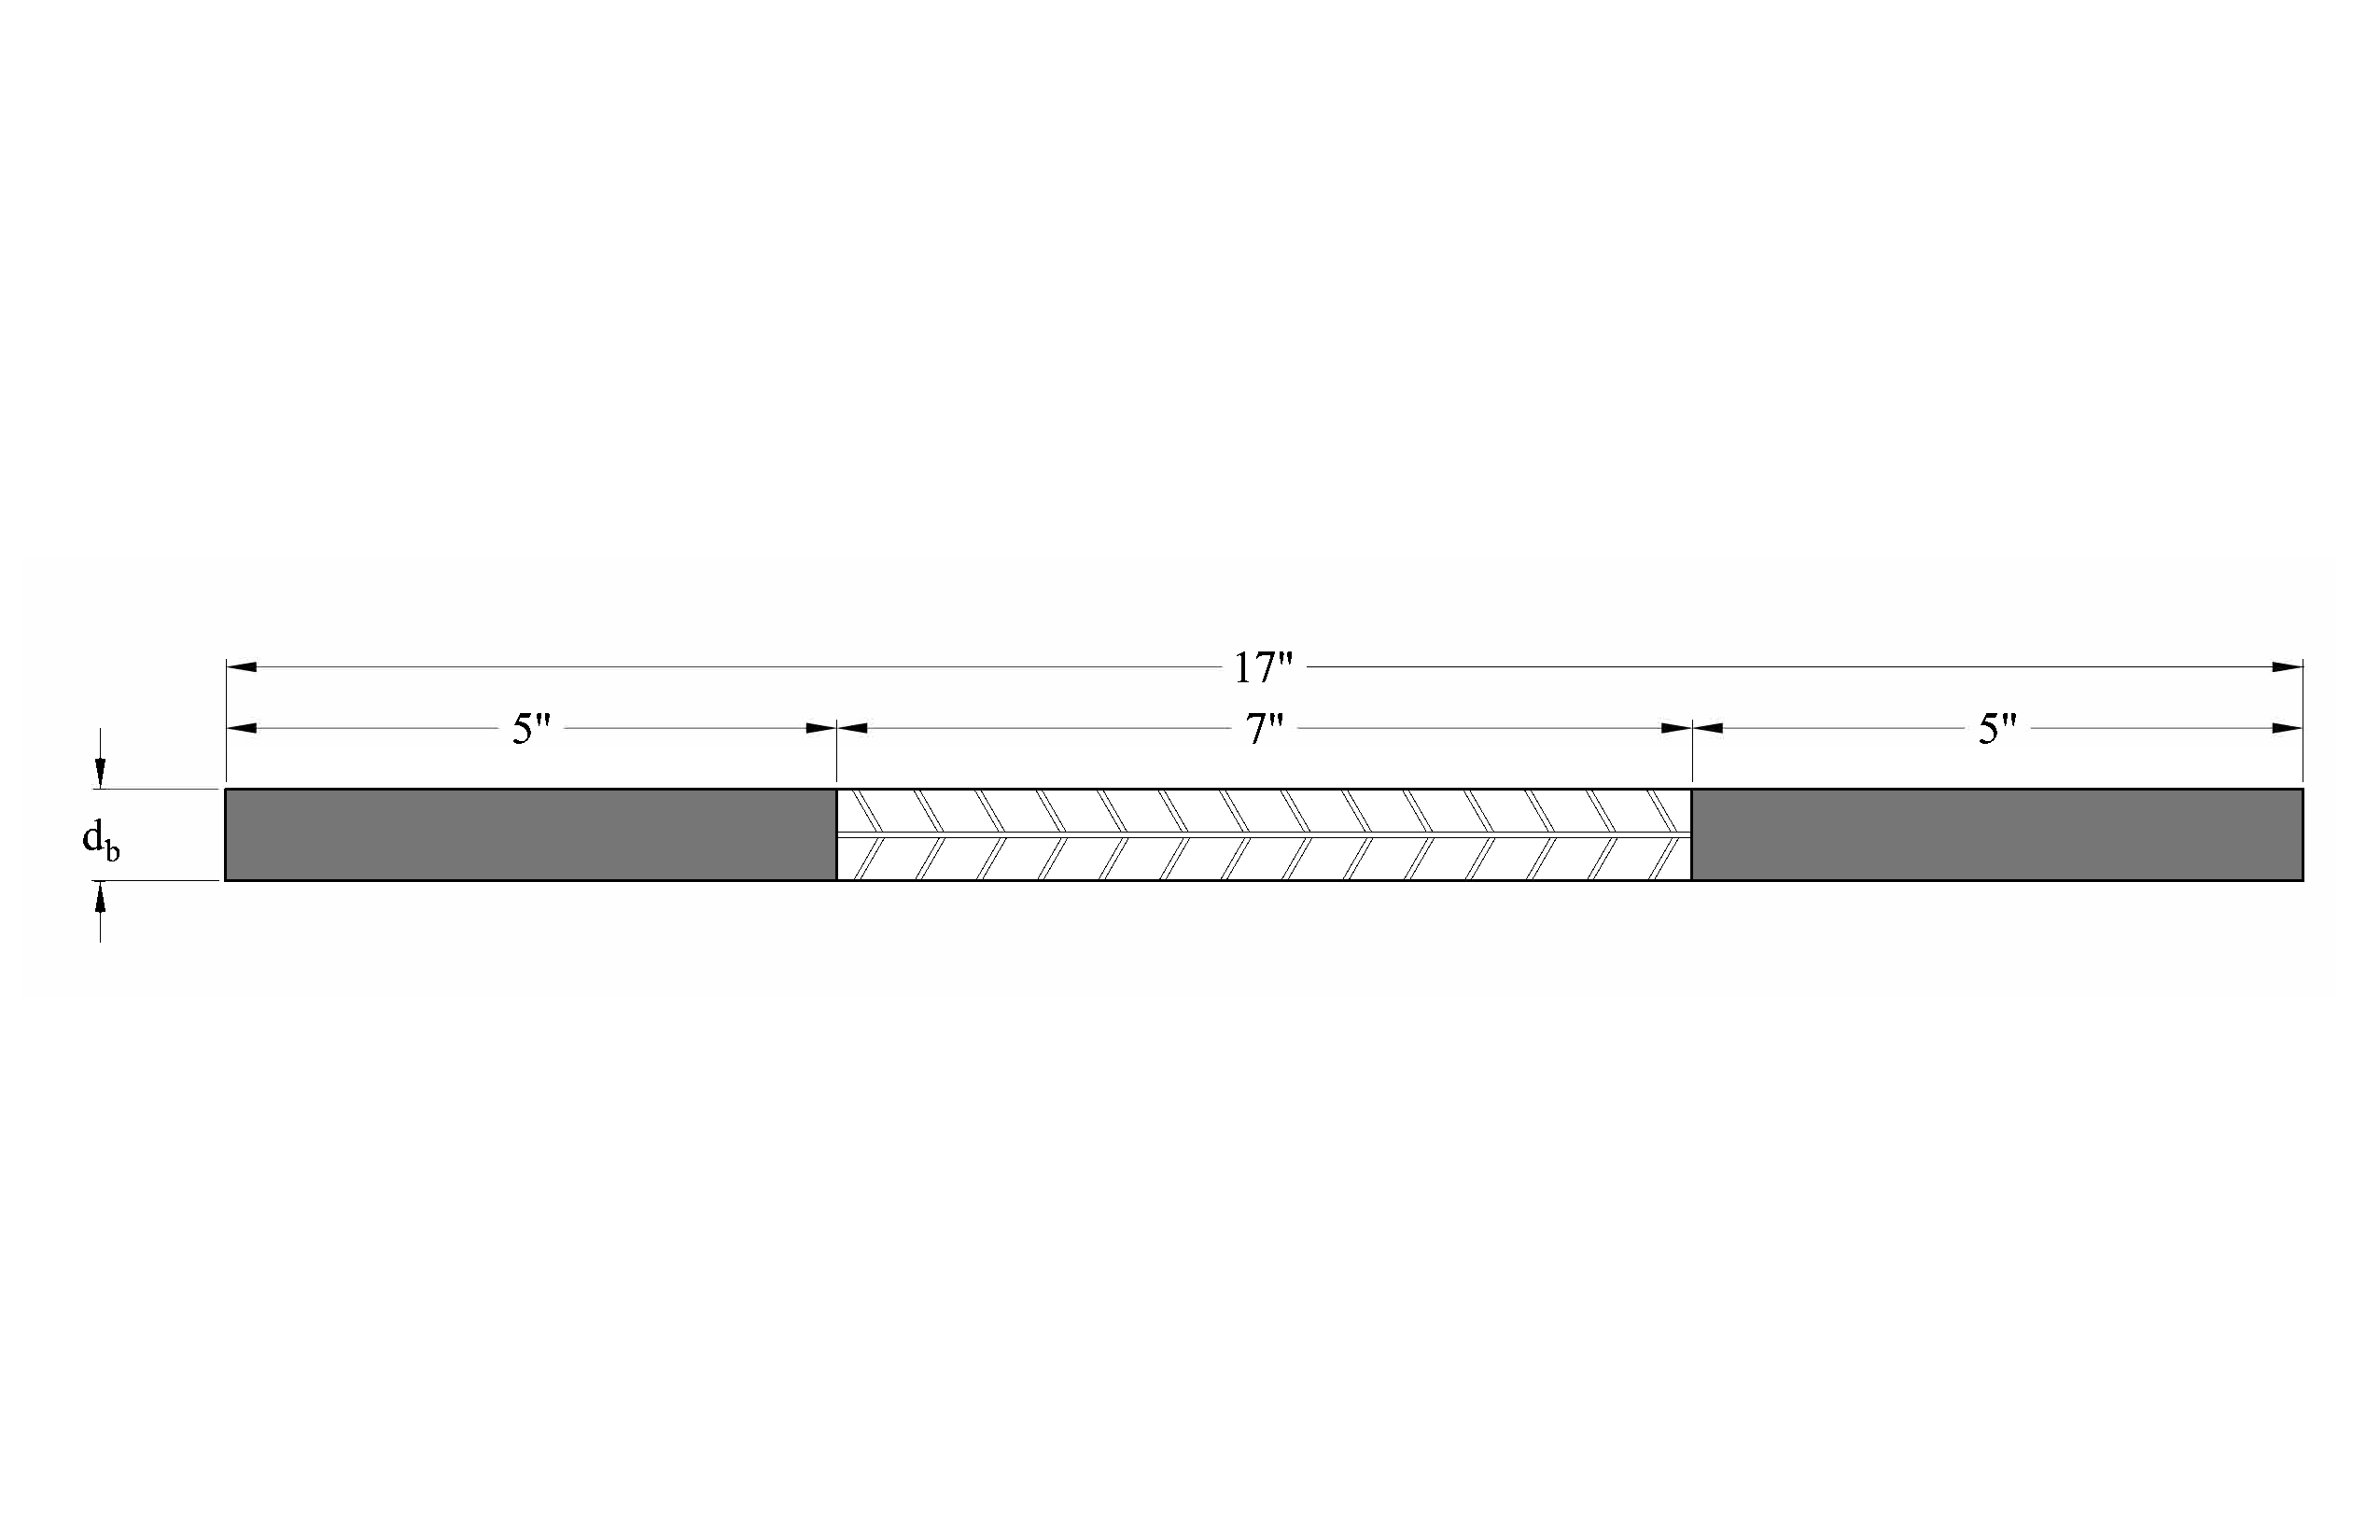
\includegraphics[width=1.0\textwidth]{Chapter-3/figs/RebarSamples}
	\caption{Rebar Specimen Geometry}
	\label{fig:RebarSpecimenGeomtry}
\end{figure}

\begin{figure}[htbp]
	\centering
	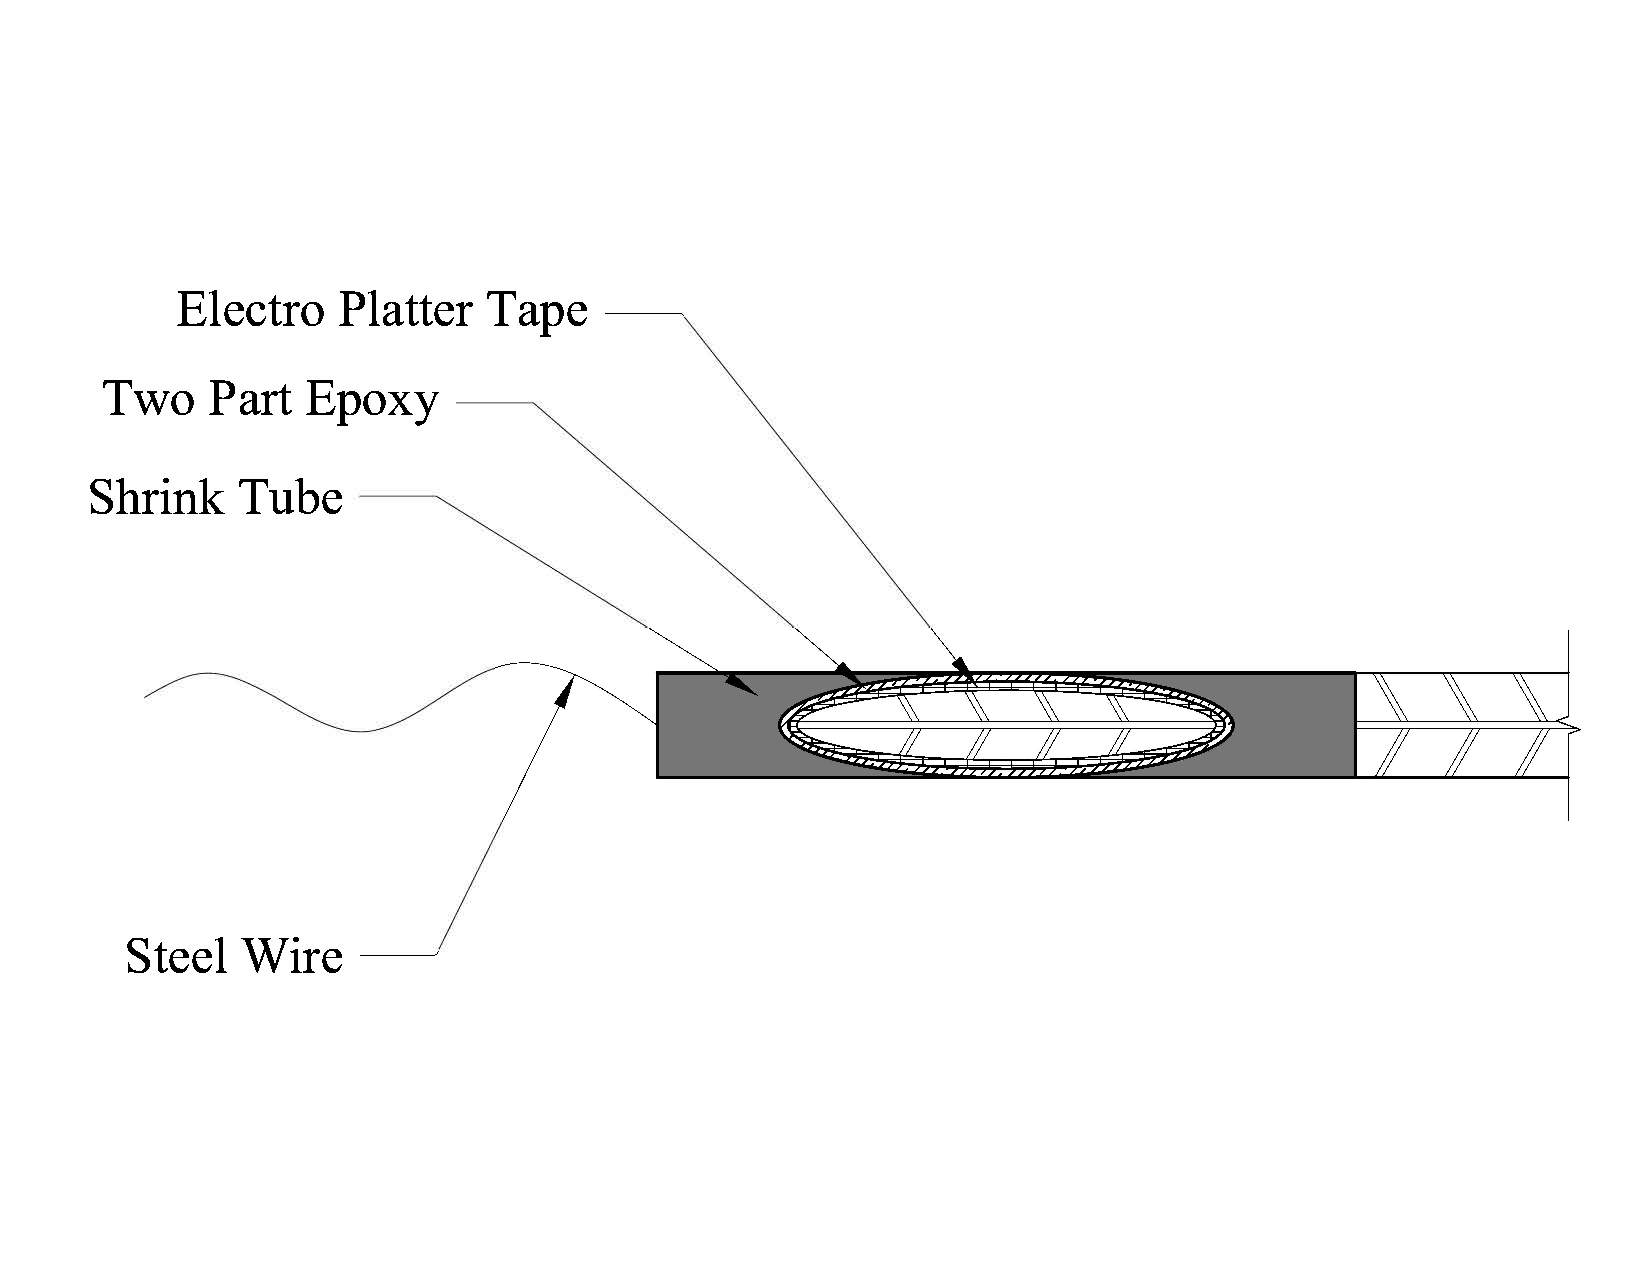
\includegraphics[width=0.7\textwidth]{Chapter-3/figs/Rebar_Ends}
	\caption{Rebars Ends Protection}
	\label{fig:RebarEndsProtection}
\end{figure}
\newpage 

To optimize the space and time it takes to prepare the rebars for corrosion, a large parent rebar that contains three specimens was prepared. This ensured that the parent specimen, placed in a corrosion cell, provided the same level of corrosion to all the specimen subsets. After each parent specimen had the specified level of corrosion, the large specimen was cut into the three smaller specimens shown in \fref{fig:LargeSpecimen}.

\begin{figure}[htbp]
	\centering
	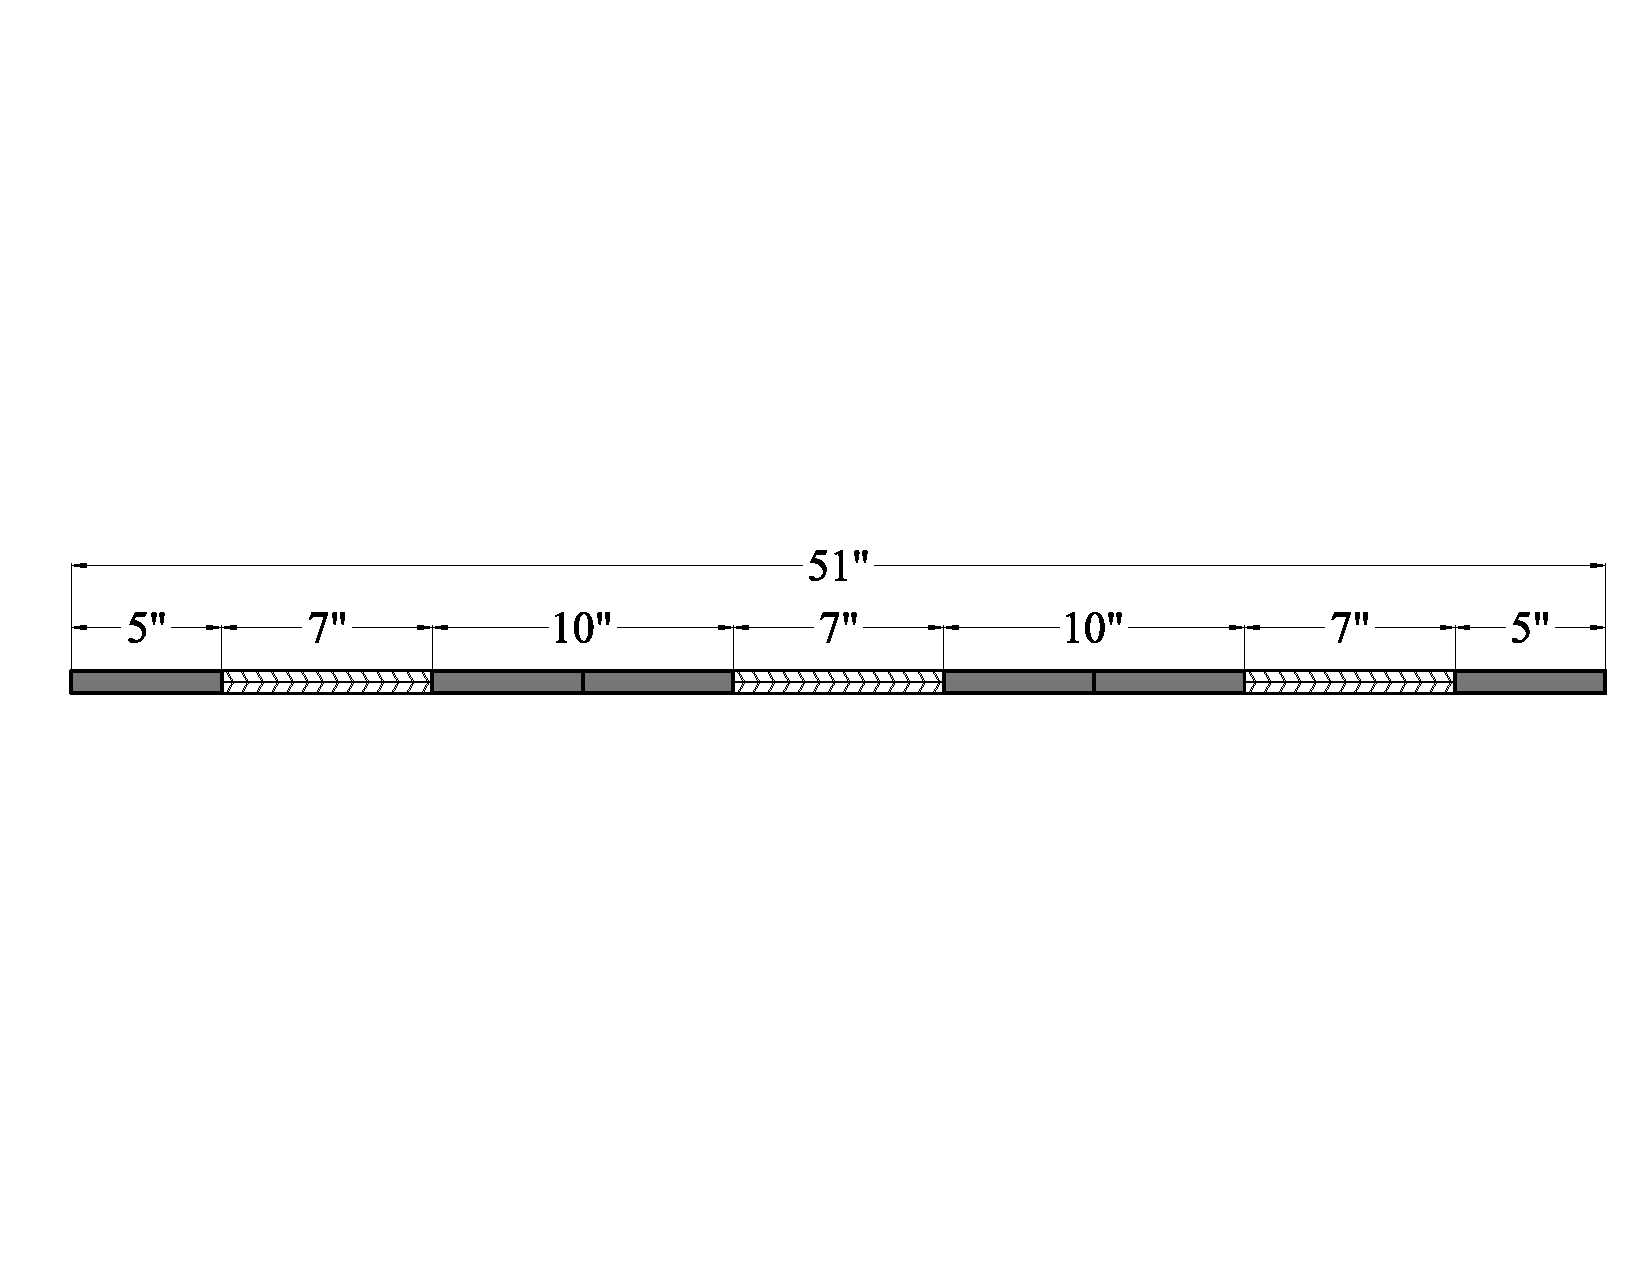
\includegraphics[width=1.0\textwidth]{Chapter-3/figs/LargeSpecimen}
	\caption{Large specimen containing three subset of specimens}
	\label{fig:LargeSpecimen}
\end{figure}

\subsection{Passivation of Rebar Specimens}

In order to simulate the conditions of rebars embedded in concrete, it was necessary to generate the passive layer on the surface of the rebars. There are two ways to generate the passive layer: (1) embed rebars in concrete and wait for the passive layer to generate, or (2) submerge the reinforcing steel in a synthetic pore solution that mimics the cement paste environment. The second option is more suited for material testing, since it does not involve demolishing the concrete. To this regard, Ghods et al \cite{Ghods2010} developed ten different pore solutions to generate the passive film on the surface of rebars. The pore solutions that were developed in their study intended to mimic the cement paste. Their study conducted 10 solutions designed to encompass concentrations of $Ca^{+2}$, $Na^{+}$, $K^{+}$, and $(SO_{4})^{+}$ found in the cement paste. The solution that generated the passive layer with the best quality of protective film, based on passive current density, was used in this study. To achieve the desired concentration of the $Ca^{+2}$, $Na^{+}$, $K^{+}$, and $(SO_{4})^{+}$ ions, the following concentration of chemicals recommended in \cite{Ghods2010} was used in the pore solution:

\begin{itemize}
	\item Saturated calcium hydroxide $Ca(OH)_2$ (approx. 1.7 g/L)
	\item Sodium hydroxide $Na(OH)$ (4.00 g/l)
	\item Potassium hydroxide $(KOH)$ (11.22 g/l)
	\item Calcium sulfate dehydrate $Ca(SO)_4 + 2H_2O$ (13.77 g/l)
\end{itemize}

The rebars were placed in the pore solution as received without any special surface preparation in the gauge length, since any  form of special surface preparation affects the quality of  the passive layer \cite{Andersson1989}, \cite{DawnMarcotte2001}, \cite{Moragues1987}, and \cite{Page1983}. In addition, Ghods et al showed no significant change in the anodic polarization of the rebar surface after being placed in the pore solution for 8 days or 14 days. Their results are shown in \fref{fig:GhodsRebarPassivation}. Therefore, the rebars were placed in the pore solution for a minimum of 8 days. 

\begin{figure}[htbp]
	\centering
	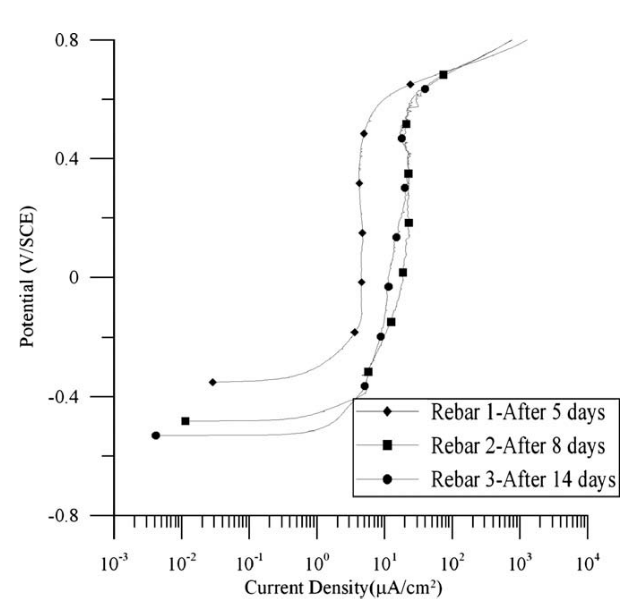
\includegraphics[width=0.6\textwidth]{Chapter-3/figs/AsReceived_AnodicPolarization_time}
	\caption{As received rebars anodic polarization immersed in pore solution for different times\cite{Ghods2009}}
	\label{fig:GhodsRebarPassivation}
\end{figure}

A specimen preparation assembly was constructed to prepare the rebars for the development of the passive layer. The assembly consisted of placing the rebar inside a PVC pipe, closing the ends of the pipe with a $90^{\circ}$ PVC elbow, and closing the open ends with PVC pipe plugs. The assembly is shown in \fref{fig:RebarPassivation}. This assembly ensured that the pipe remained airtight and prevented the carbonation of the calcium hydroxide ($Ca(OH)_{2}$ in the pore solution.

\begin{figure}[htbp]
	\centering
	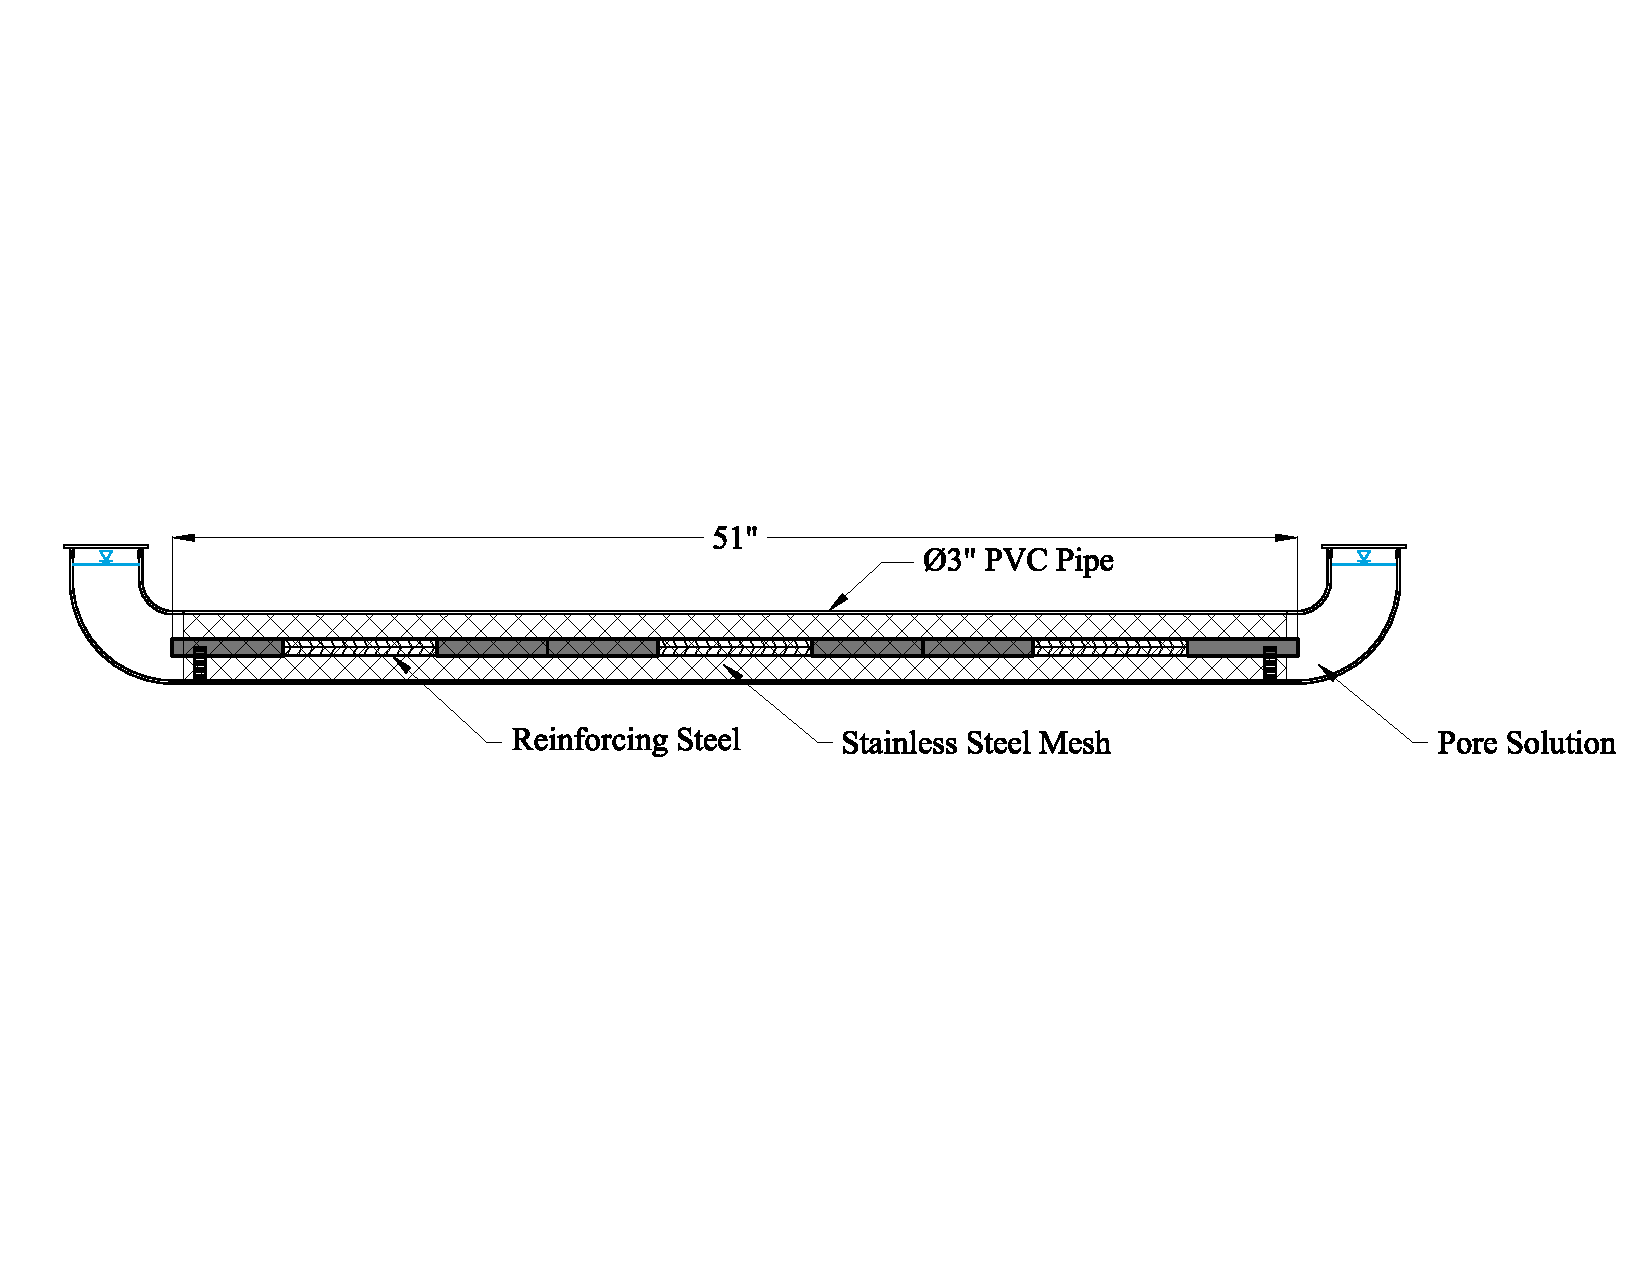
\includegraphics[width=1.0\textwidth]{Chapter-3/figs/AnodicPolarization_01}
	\caption{Assembly for rebar preparation for the development of passive layer in pore solution}
	\label{fig:RebarPassivation}
\end{figure}

\subsection{Accelerated Corrosion  of Rebars}

Four components are required for corrosion to occur: (1) the anode, (2) the cathode, (3) an electrolytic connection, and (4) an electrical path. The corrosion cell deployed in this study   used this concept in the following way:  the anode consisted of the rebar, the cathode consisted  of a stainless steel mesh, the electrolytic connection was made with a sodium chloride solution, and the electrical path was forced via an electric circuit. The corrosion cell uses the assembly developed to generate the passive layer with the components needed for corrosion as shown in \fref{fig:AcceleratedCorrosion}. The circuit was  designed so that the current in the specimen was $150 mA$, equivalent to $340 \mu A/cm^2$ on the gauge length surface of the rebar. To the author's knowledge this is the lowest current density ever used on an accelerated corrosion process for corroded rebars subjected to tension and BBT tests. Since the rebar and stainless steel mesh have a low resistance, a $100 \Omega$ resistor was added to the circuit, such that it stabilized the current and kept it constant at $150mA$.

\begin{figure}[htbp]
	\centering
	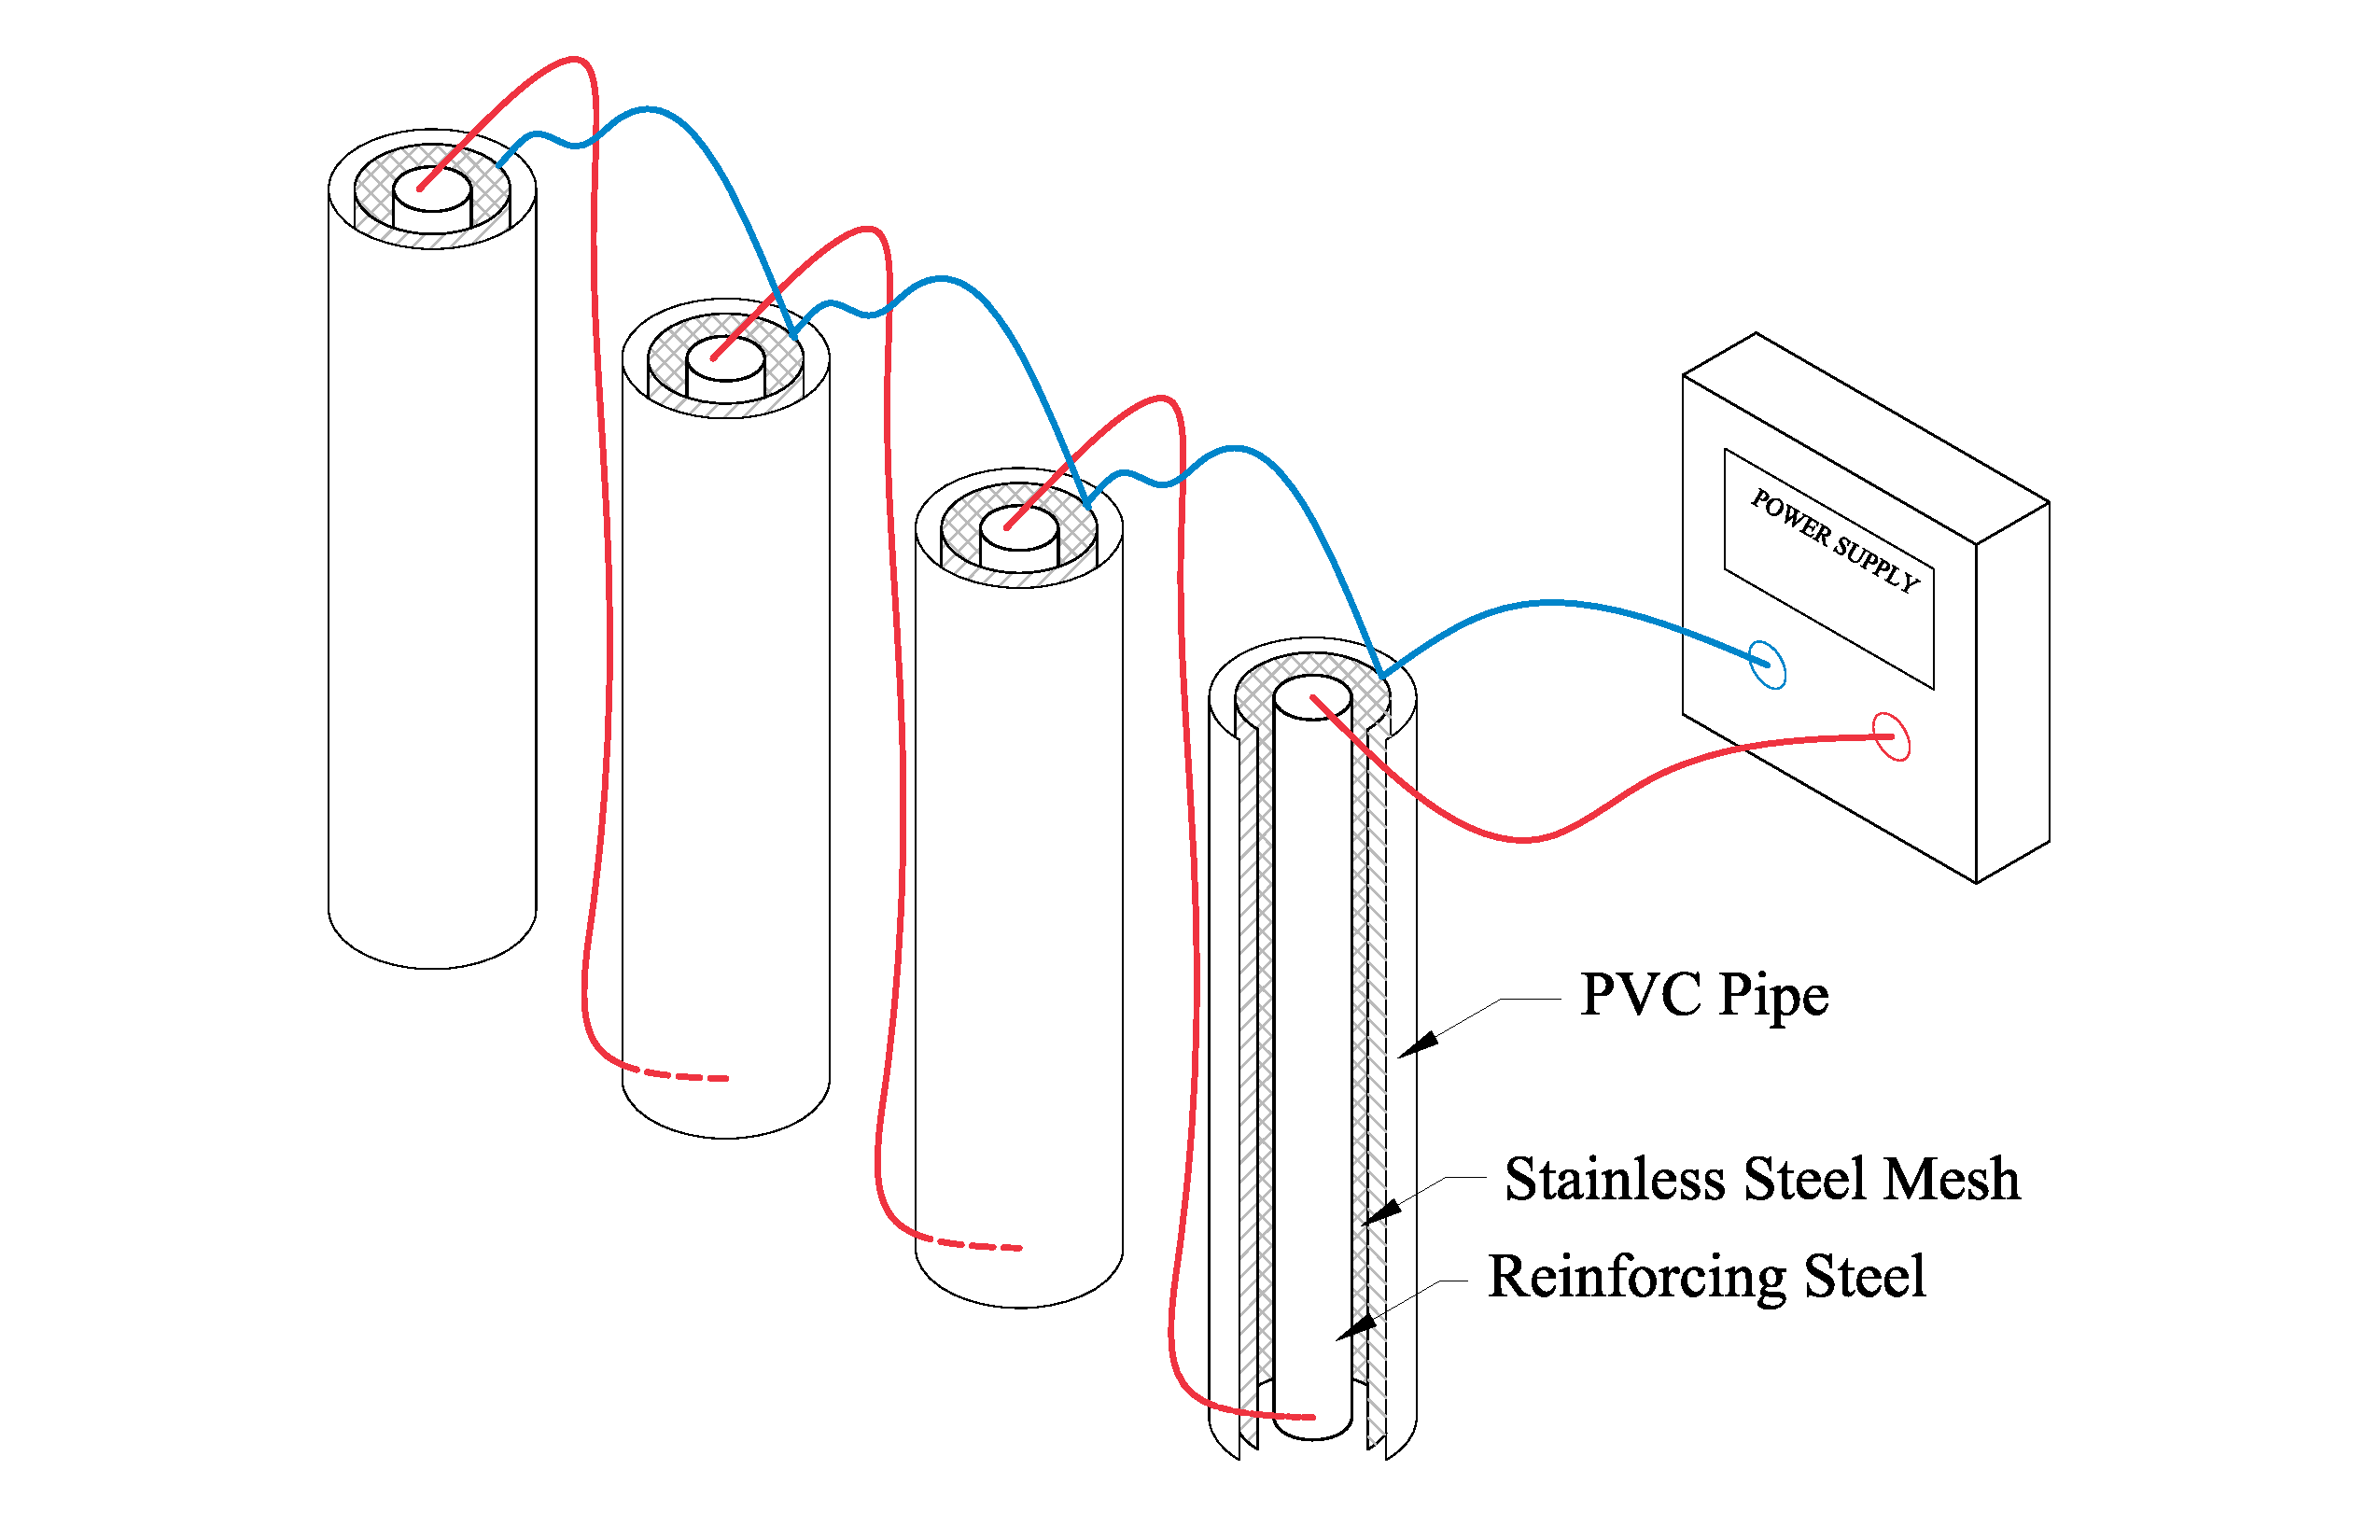
\includegraphics[width=0.95\textwidth]{VAC Prelim 2.0/Chapter-3/figs/AcceleratedCorrosionProcedure.pdf}
	\caption{Accelerated corrosion process}
	\label{fig:AcceleratedCorrosion}
\end{figure}

Ghods et al \cite{Ghods2010} determined that for rebars with passive films, a concentration of 0.3 Moles of sodium chloride ($NaCl$) will start the depassivation process on the rebars. Accordingly the same sodium chloride solution was used in this study. To estimate the time to apply the current and obtain the desired level of corrosion, Faraday's law shown in \eref{eq.FaradayEq} was used.

\begin{equation}
	m_{loss}=\frac{it(AM)}{nF}
	\label{eq.FaradayEq}
\end{equation}

 In \eref{eq.FaradayEq}, $m_{loss}$ corresponds to the mass loss, $i$ is the current in amperes ($i=5 mA$), $t$ is the time the current is sustained in seconds, and $(AM)$ is the atomic mass of the oxidizing component. For this study the oxidizing component is the iron ($Fe$) in the rebars, hence $(AM)=54.845g/mol$, $n$ is the number of electrons lost per atom oxidized, for iron ($Fe$) the number of electrons is equal to 2, and $F$ is Faraday's number ($F=96485 C$). Solving \eref{eq.FaradayEq} for $t$ and assuming uniform corrosion for different corrosion levels, the time of application was calculated for the total gauge length in the parent rebar specimen. The estimated times to achieve the corrosion levels are shown in Table \ref{tab:AcceleratedCorrosionTime}. 

\begin{table}[htbp]
	\caption{Accelerated corrosion times for the total length in parent specimen of a 19 mm (0.75 in) rebar}
	\label{tab:AcceleratedCorrosionTime}
	\centering	
		\begin{tabular}{l c c}
		Corrosion Level (CL) & Mass loss (g)   & time (days)     \\  \hline	
		5\%                  & 57.6            & 16    \\	
		10\%                 & 115.3            & 31     \\	
		15\%                 & 172.9            & 47   \\	
		20\%                 & 230.5            & 63     \\
		25\%                 & 288.1               & 78   \\
		\end{tabular}
\end{table}

After the accelerated corrosion is performed, the corrosion products from the bar are removed via a hydrochloric acid application. The acid removes imperfections on the surface and allows the placement of the instrumentation on the surface of the reinforcing steel bar.

\section{Tension Tests}

The tension tests were performed to evaluate differences in the stress-strain behavior of corroded reinforcing steel with those found in the literature. In addition, the data obtained from these tests served as an input to the analytical model. The tension tests were performed in accordance with the standard ASTM A370, which specifies the loading procedure and the gauge lengths. 
\subsection{Tension Test Procedure}

The tension tests consisted of:
\begin{enumerate}
    \item Placing the rebar in the universal testing machine
    \item Pulling the rebar in tension 
    \item Recording the load and the strain on the rebar 
\end{enumerate}

The strains were captured through the use of LED markers from the Optrotrak Certus HD system. The gauge length between the LED markers was 2 inches as is specified in the ASTM A370 standard. \fref{fig:TensionTest} shows an example of the test setup. The stress was calculated based on the load reading from the UTM machine and divided by the measured area of the corroded rebars.

\begin{figure}[htbp]
	\centering
	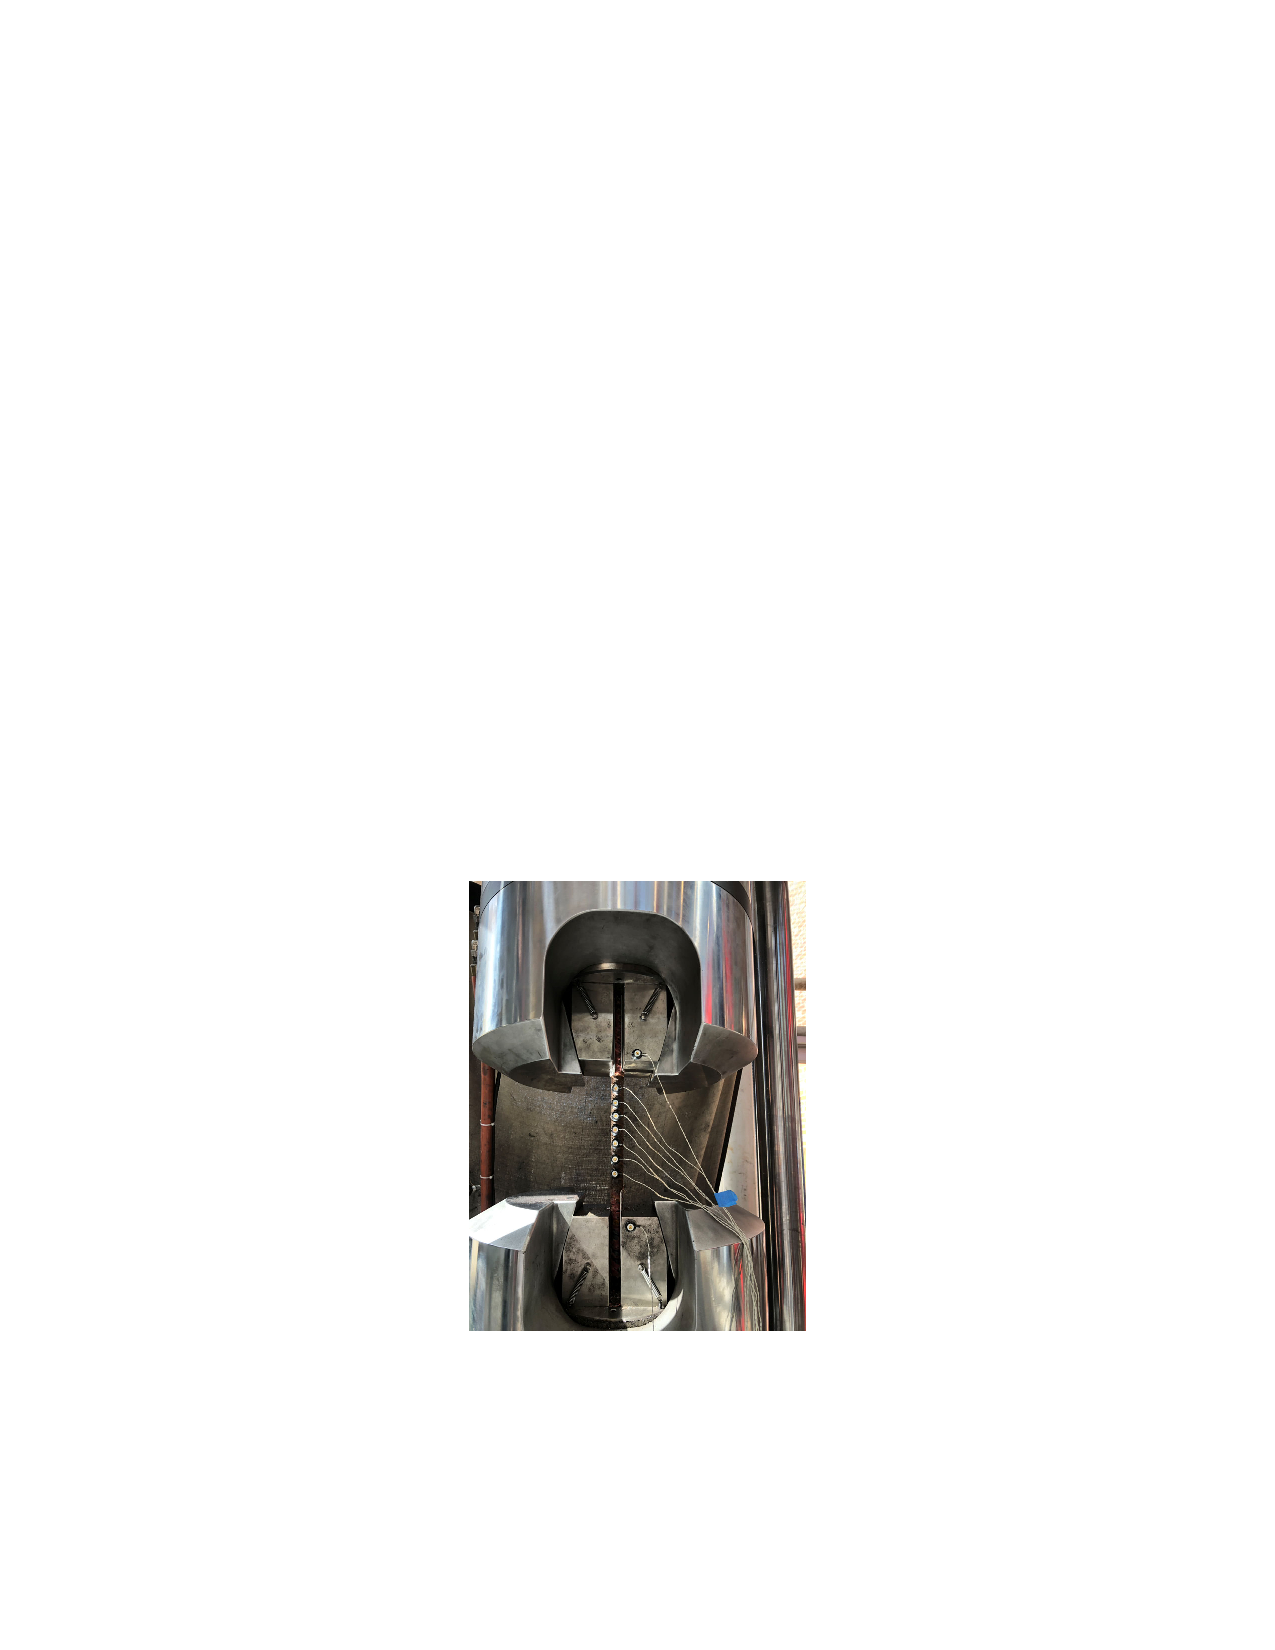
\includegraphics[width=0.4\textwidth]{VAC Thesis 2.0/Chapter-3/figs/tension_test_utm.pdf}
	\caption{Tension test setup}
	\label{fig:TensionTest}
\end{figure}

\subsection{Testing Parameters}
The results obtained from the tension tests were valuable to understanding the change in the stress-strain relationship, the yield strength, and ultimate strength of corroded rebars. These values were obtained as outlined in ASTM A370, and are summarized below.

\textbf{Yield Strength}: Yield strength is the stress at which a material exhibits a specified limiting deviation from the proportionality of stress to strain. To determine the yield strength, the offset method was used to obtain this value.

\textbf{Ultimate Strength}: Ultimate strength is calculated by dividing the maximum load the specimen sustains during a tension test by the original cross-sectional area of the specimen.

\textbf{Uniform Axial Elongation}: The elongation is the increase in length of the gauge length, expressed as a percentage of the original gauge length.

Regression analysis of the results helped update the equations that correlate these parameters to the corrosion level, and yielded an updated form of \eref{eq.eleven}. The outcomes of the tension tests informed the results of the analytical model in Chapter \ref{chap-five}.

\subsection{Test Matrix}

A total of 3 tension tests per corrosion level were envisioned for each corrosion level from 0\% - 20\%. The specimens were labeled in accordance with the the following format:

$CL-$ (Corrosion level in  \%) $-T-$ Subset specimens (initial specimen\_final specimen)

It must be noted, as will be shown in the results in Chapter \ref{chap-four}, that the specimen for CL=15\% did not reach the intended corrosion level, mainly due to a faulty weld between the stainless steel wire and the specimen. The intended test matrix is presented in \ref{tab:tension_matrix}.

\begin{table}[htbp]
\caption{Tension test matrix}
\label{tab:tension_matrix}
\centering
\begin{tabular}{lccl}
Parent specimen label        & Target CL (\%)      & Initial mass (g)        & Subset specimen label \\ \hline
\multirow{3}{*}{CL5-T-1\_3}  & \multirow{3}{*}{5}  & \multirow{3}{*}{1260.8} & CL-5-T-1              \\
                             &                     &                         & CL-5-T-2              \\
                             &                     &                         & CL-5-T-3              \\
\multirow{3}{*}{CL10-T-1\_3} & \multirow{3}{*}{10} & \multirow{3}{*}{1244.0} & CL-10-T-1             \\
                             &                     &                         & CL-10-T-2             \\
                             &                     &                         & CL-10-T-3             \\
\multirow{3}{*}{CL15-T-1\_3\*} & \multirow{3}{*}{15} & \multirow{3}{*}{1251.2} & CL-15-T-1             \\
                             &                     &                         & CL-15-T-2             \\
                             &                     &                         & CL-15-T-3             \\
\multirow{3}{*}{CL20-T-1\_3} & \multirow{3}{*}{20} & \multirow{3}{*}{1251.2} & CL-20-T-1             \\
                             &                     &                         & CL-20-T-2             \\
                             &                     &                         & CL-20-T-3            
\end{tabular}
\end{table}

\section{Buckled Bar Tension (BBT) Tests}

One of the limit states considered in the seismic design of bridge columns is the fracture of buckled rebar, which corresponds to the ultimate limit state. Recent tests have been developed to determine the critical bending strain of buckled reinforcing steel \cite{Barcley2019}, which is associated with the sudden fragile fracture of buckled longitudinal reinforcement of RC columns. The buckled bar tension (BBT) test simulates the bending and tension strain demands on a buckled bar to determine critical bending strain of buckled rebars. 

\subsection{Test Procedure}
Barcley et al \cite{Barcley2019} developed a methodology to calculate local strains on a buckled bar using an LED optical sensor system \cite{NorthernDigitalInc.2020}. \fref{fig:BBTseq} shows the basic concept of the BBT test.

\begin{figure}[htbp]
	\centering
	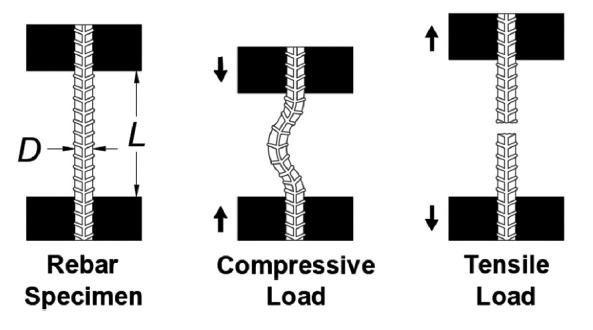
\includegraphics[width=0.7\textwidth]{Chapter-3/figs/BBT_Sequence}
	\caption{BBT test sequence\cite{Barcley2019}}
	\label{fig:BBTseq}
\end{figure}

The procedure to perform the buckled bar tension test consisted of:

\begin{enumerate}
    \item First, the rebar was placed in the universal testing machine (UTM), and the corroded rebar specimen was prepared with LED markers on the surface, such that the displaced shape of the bar could be measured.
    \item Second, the rebar specimen was compressed to impose a bending strain of a prescribed level. Barcley et al showed that a fourth order polynomial can be fit to the LED sensors near the buckled region of the bar to obtain the displaced shape ($w$). The bending strain was calculated using solid mechanics principles. The curvature is the second derivative of the displaced shape ($w$) for small displacements, which is calculated as: 
    \begin{equation}
        \phi=\frac{\frac{d^2w(x)}{dx^2}}{\left[1+\left(\frac{dw(x)}{dx}\right)\right]^\frac{3}{2}}\approx \frac{d^2w(x)}{dx^2}
        \label{eq.CuvatureAprox}
    \end{equation}
    If we assume that the bending is symmetric for the rebar then the strain in the extreme fibers of the rebar is calculated as:
    \begin{equation}
        \varepsilon_{b}=\phi\left(\frac{d_{bl}}{2}\right) 
        \label{eq.BendingStrain}
    \end{equation}    
    Combining \eref{eq.CuvatureAprox}, and \eref{eq.BendingStrain}, the bending strain can be expressed as:
    \begin{equation}
        \varepsilon_{b}=\frac{d^2w(x)}{dx^2}\left(\frac{d_{bl}}{2}\right) 
        \label{eq.BendingStrainExpanded}
    \end{equation}
    An example of the calculation of the bending strain is shown in \fref{fig:BBT_Curvature}
    \item Third, once buckled to the prescribed curvature, the bar is loaded in tension until fracture is observed
    \item 4.	Then the process was repeated with a different bar for a different bending strain. After all the tests were performed, results from elongation at peak force were generated as in the example shown in  \fref{fig:BBT_MaxBendingStrain}. The critical bending strain was determined from the results obtained through BBT tests. The critical bending strain is defined as the point at which a low elongation under load is obtained. This low elongation results in a brittle fracture of the rebar as shown in \fref{fig:BBT_DuctileBrittle}(b). \fref{fig:BBT_MaxBendingStrain} shows that for pristine rebars of grade 80 ksi steel the critical bending strain is $\varepsilon_{b,0}=0.14$.
\end{enumerate}

\begin{figure}[htbp]
    \centering
    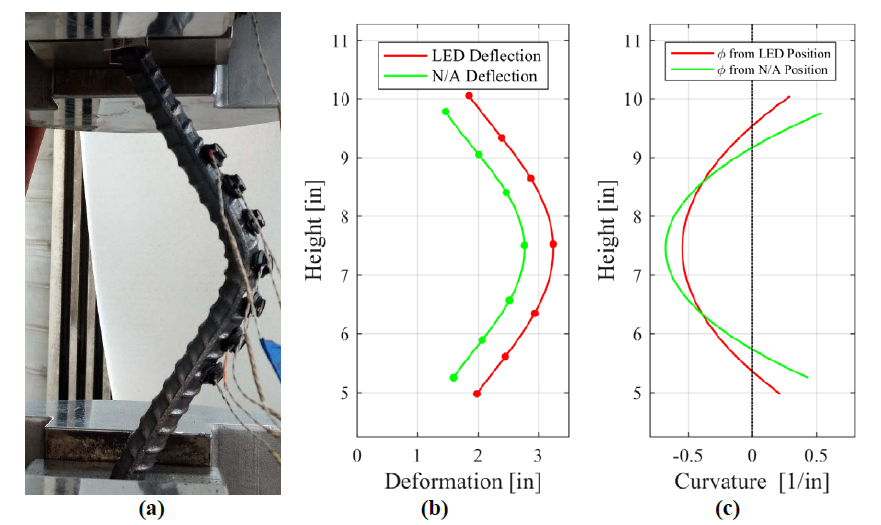
\includegraphics[width=0.8\textwidth]{Chapter-3/figs/BBT_Curvature}
    \caption{a) Picture of buckled bar; (b) Position of optical markers and adjustment to neutral axis; (c) Calculation of curvature \cite{Barcley2018}}
    \label{fig:BBT_Curvature}
\end{figure}
\begin{figure}
    \centering
    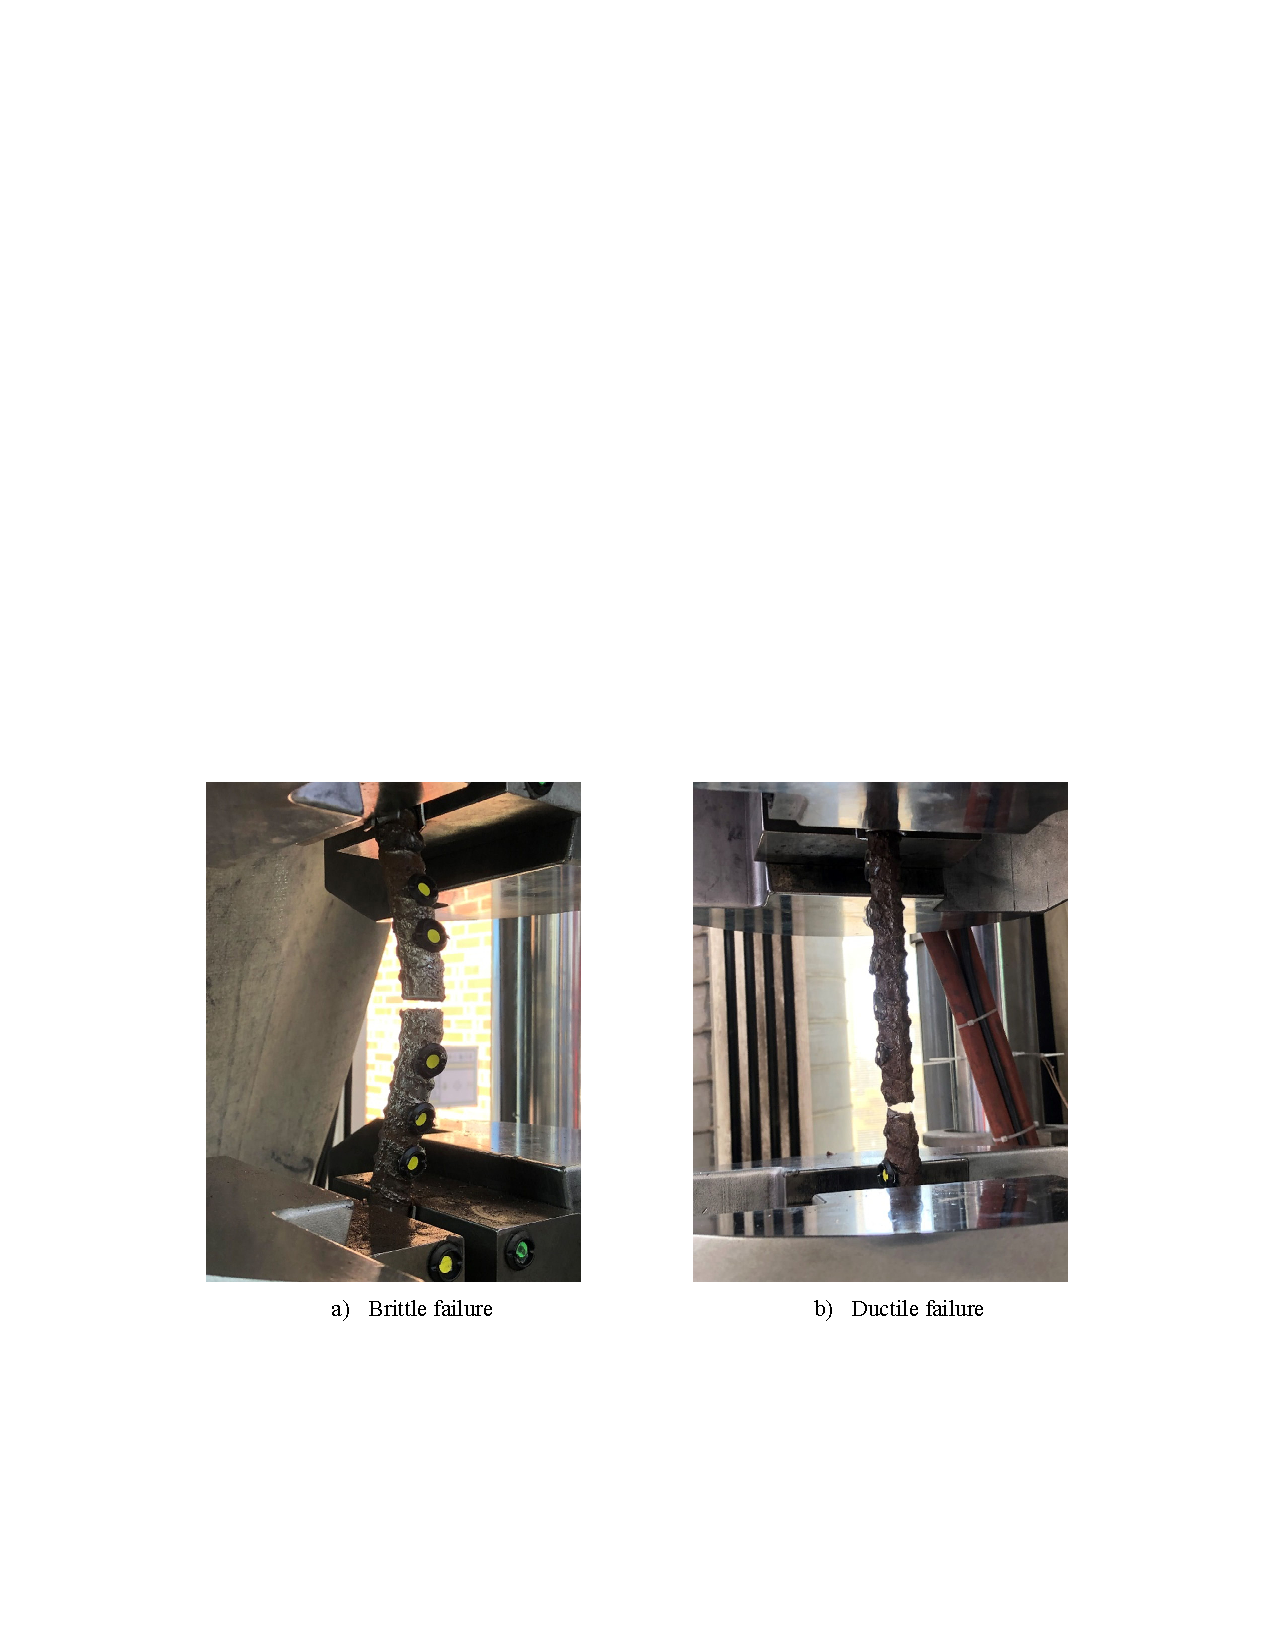
\includegraphics[width=1.0\textwidth]{VAC Thesis 2.0/Chapter-3/figs/bbt_ductile_vs_brittle.pdf}
    \caption{(a)Ductile rebar fracture; (b) Brittle rebar fracture}
    \label{fig:BBT_DuctileBrittle}
\end{figure}
\begin{figure}[htbp]
    \centering
    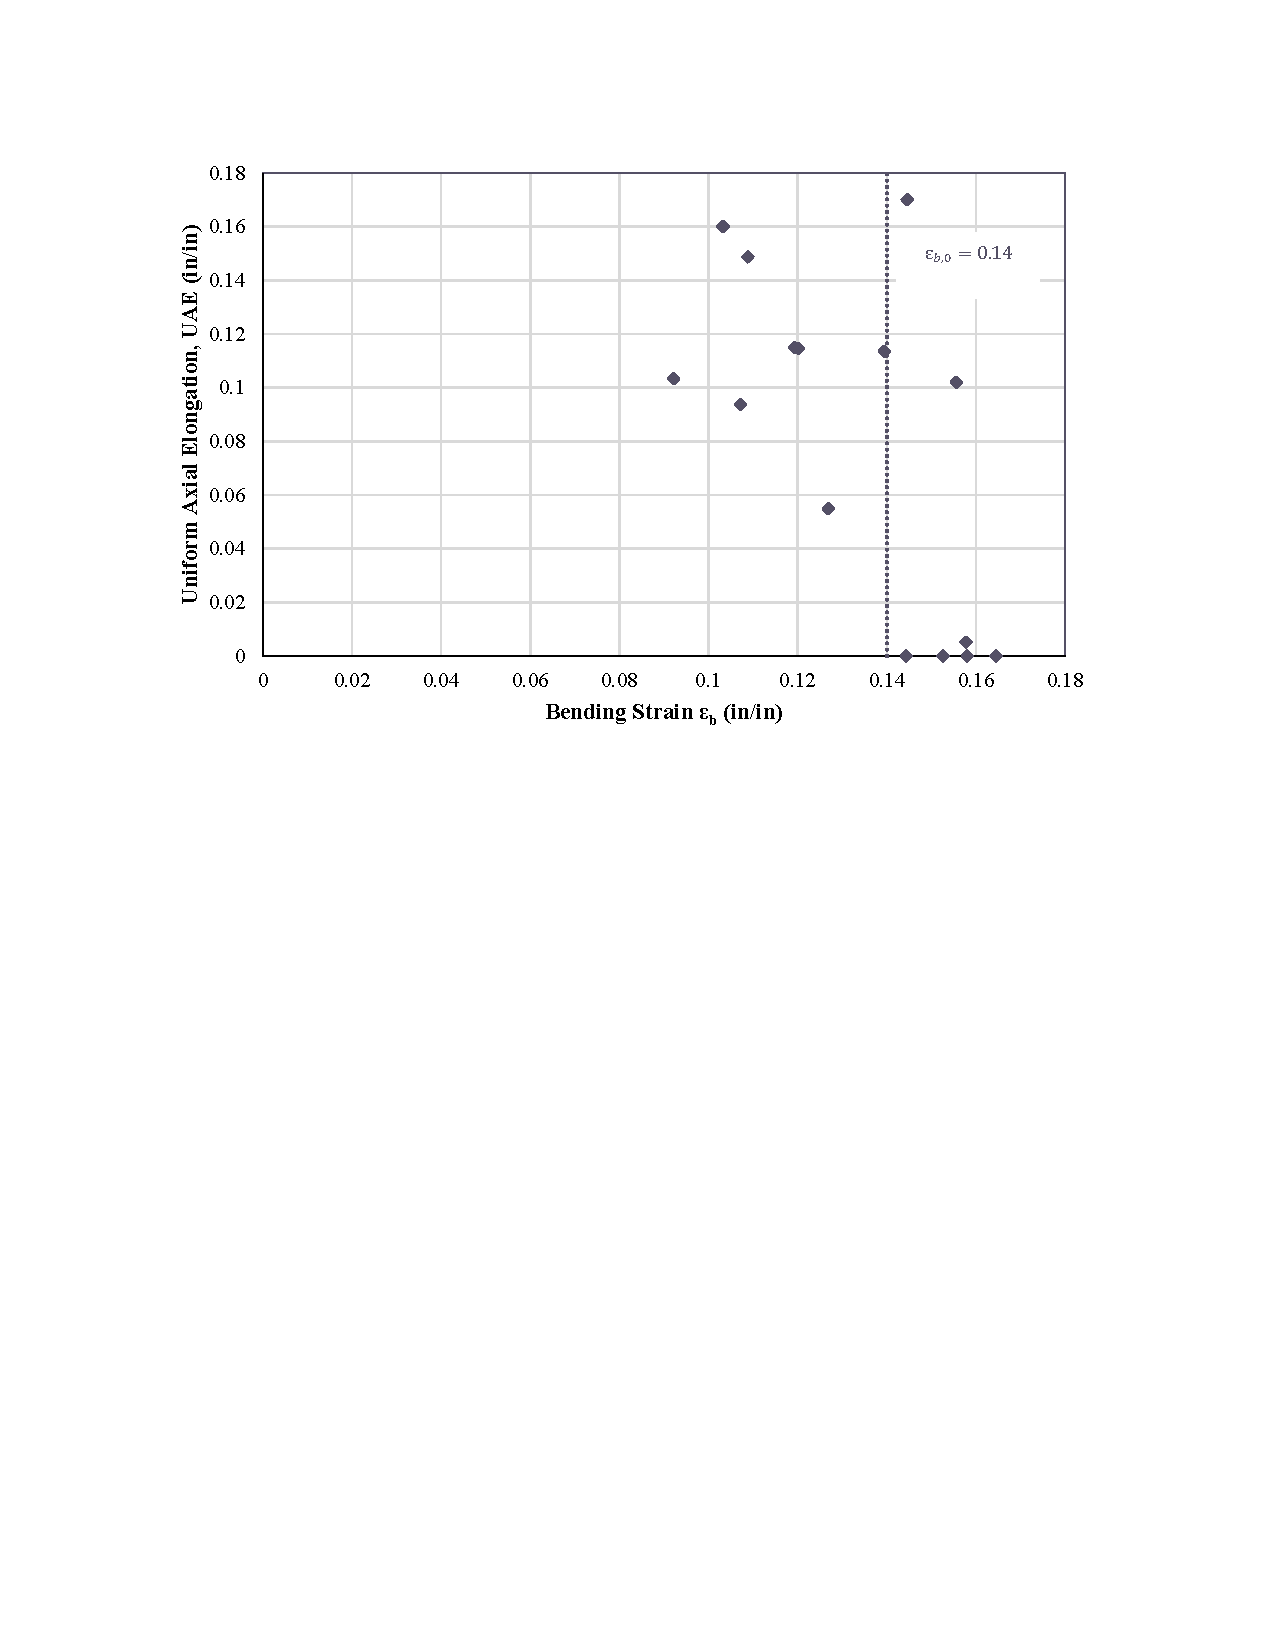
\includegraphics[width=0.9\textwidth]{VAC Thesis 2.0/Chapter-3/figs/bbt_bendinstrain_cl0.pdf}
    \caption{BBT results for pristine rebars \cite{Barcley2018}}
    \label{fig:BBT_MaxBendingStrain}
\end{figure}

\newpage

\subsection{Testing Parameters}

The main parameter obtained from the BBT test was the maximum bending strain. As previously defined, the maximum bending strain defines the maximum level of buckling a rebar can sustain before reaching a brittle failure, and set the ultimate limit state of reinforced concrete members.

\textbf{Maximum bending strain}: This parameter was obtained at the sudden drop in elongation capacity of a bar is subjected to buckling and later pulled. At  this level of bending strain, the type of fracture becomes brittle and thus no elongation of the specimen occurs.

\subsection{Test Matrix}
The BBT tests matrix deployed in this research is shown in Table \ref{tab:bbt_matrix}. A total of 30 tests were performed, six tests for corrosion levels ranging from 0\%-20\%. The specimens were labeled in accordance with the following format:
\newline
$CL$-(Corrosion level in  \%)$-BBT-$ Subset specimens (initial specimen\_final specimen)

\begin{table}[htbp]
\caption{BBT test matrix}
\label{tab:bbt_matrix}
\centering
\begin{tabular}{lccl}
Parent specimen label          & Initial mass (g)        & Target CL (\%)      & Subset specimen label \\ \hline
\multirow{3}{*}{CL5-BBT-1\_3}  & \multirow{3}{*}{1249.6} & \multirow{3}{*}{5}  & CL-5-BBT-1            \\
                               &                         &                     & CL-5-BBT-2            \\
                               &                         &                     & CL-5-BBT-3            \\
\multirow{3}{*}{CL5-BBT-4-6}   & \multirow{3}{*}{1255.3} & \multirow{3}{*}{5}  & CL-5-BBT-4            \\
                               &                         &                     & CL-5-BBT-5            \\
                               &                         &                     & CL-5-BBT-6            \\
\multirow{3}{*}{CL10-BBT-1\_3} & \multirow{3}{*}{1248.7} & \multirow{3}{*}{10} & CL-10-BBT-1           \\
                               &                         &                     & CL-10-BBT-2           \\
                               &                         &                     & CL-10-BBT-3           \\
\multirow{3}{*}{CL10-BBT-4-6}  & \multirow{3}{*}{1258.7} & \multirow{3}{*}{10} & CL-10-BBT-4           \\
                               &                         &                     & CL-10-BBT-5           \\
                               &                         &                     & CL-10-BBT-6           \\
\multirow{3}{*}{CL15-BBT-1\_3} & \multirow{3}{*}{1217.9} & \multirow{3}{*}{15} & CL-15-BBT-1           \\
                               &                         &                     & CL-15-BBT-2           \\
                               &                         &                     & CL-15-BBT-3           \\
\multirow{3}{*}{CL15-BBT-4-6}  & \multirow{3}{*}{1265.5} & \multirow{3}{*}{15} & CL-15-BBT-4           \\
                               &                         &                     & CL-15-BBT-5           \\
                               &                         &                     & CL-15-BBT-6           \\
\multirow{3}{*}{CL20-BBT-1\_3} & \multirow{3}{*}{1245.1} & \multirow{3}{*}{20} & CL-20-BBT-1           \\
                               &                         &                     & CL-20-BBT-2           \\
                               &                         &                     & CL-20-BBT-3           \\
\multirow{3}{*}{CL20-BBT-4-6}  & \multirow{3}{*}{1272.3} & \multirow{3}{*}{20} & CL-20-BBT-4           \\
                               &                         &                     & CL-20-BBT-5           \\
                               &                         &                     & CL-20-BBT-6          
\end{tabular}
\end{table}

\section{3D Scanning}

The FARO Arm \cite{FAROTechnologiesInc.2022} was used to perform 3D scans of the gauge lengths on the corroded specimens. The procedure consisted of using a probe that sends a laser signal to the surface of   the specimens. The reflections from this laser were captured by the probe and the data was acquired in a computer for later post-processing. The probe used in this research had an accuracy of 0.018 mm. The system can be seen in \fref{fig:3d_scanner_probe}.This probe is located at the the Center for Additive Manufacturing and Logistics at NC State.

\begin{figure}[htbp]
    \centering
    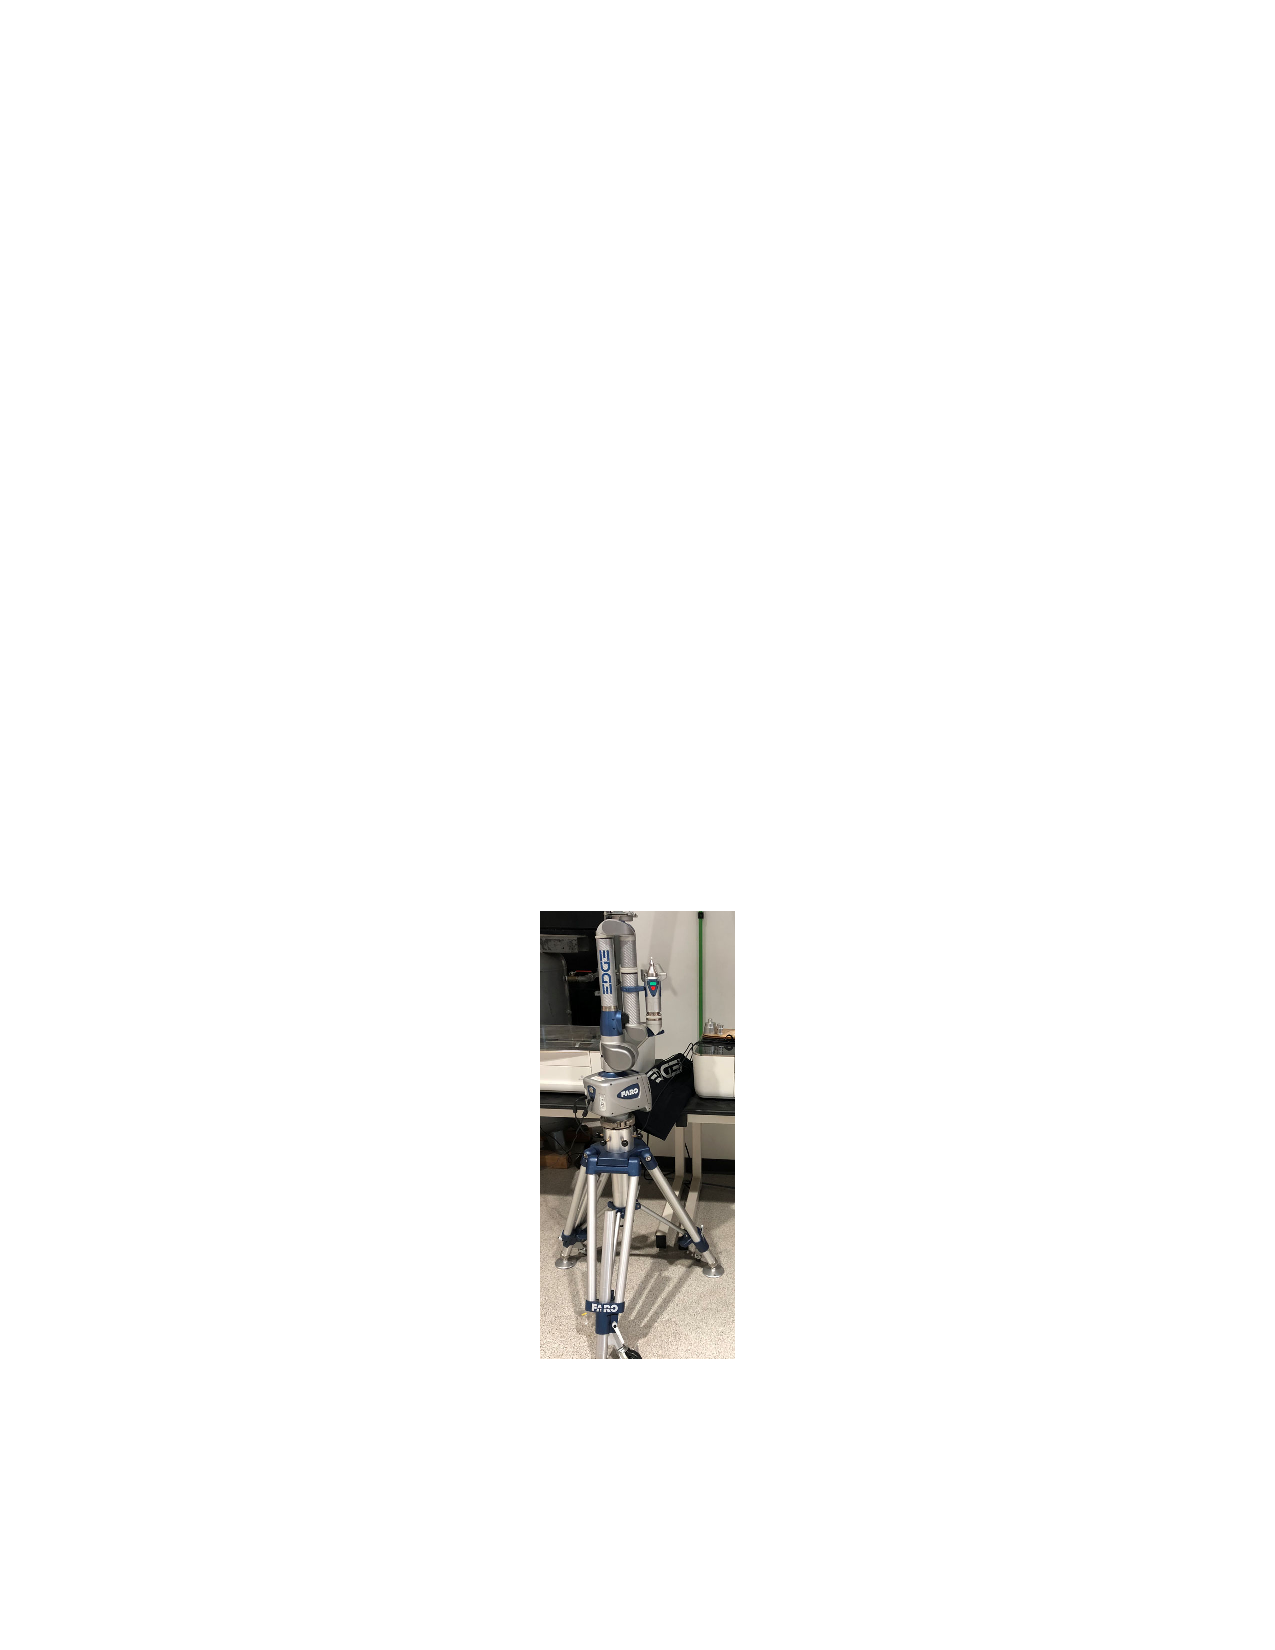
\includegraphics[width=0.2\textwidth]{VAC Thesis 2.0/Chapter-3/figs/3d_scanner_01.pdf}
    \caption{3D scan probe}
    \label{fig:3d_scanner_probe}
\end{figure}
The main use of this tool was to obtain an accurate reading of the diameter of the rebar, which provides an accurate reading of the tension and BBT tests results. The reader is referred to Chapter \ref{chap-four} to see the results obtained using this methodology. The data collected in this study can be used in future research to study the effect of imperfections using finite element analysis methods.

\section{SEM observations}

A total of six fracture surfaces were obtained from the BBT tests. Three fracture surfaces were from ductile failure, and the remaining three fracture surfaces were obtained from brittle failures. The collected fracture surfaces were observed under the Scanning Electron Microscope (SEM). In this study a Variable Pressure SEM (VPSEM) was used, since it is more suited to  studying metals. The microscope used in this study can be observed in \fref{fig:sem_photo} which is located at the Analytical Instrumentation Facility (AIF) at NC State.

\begin{figure}[htbp]
    \centering
    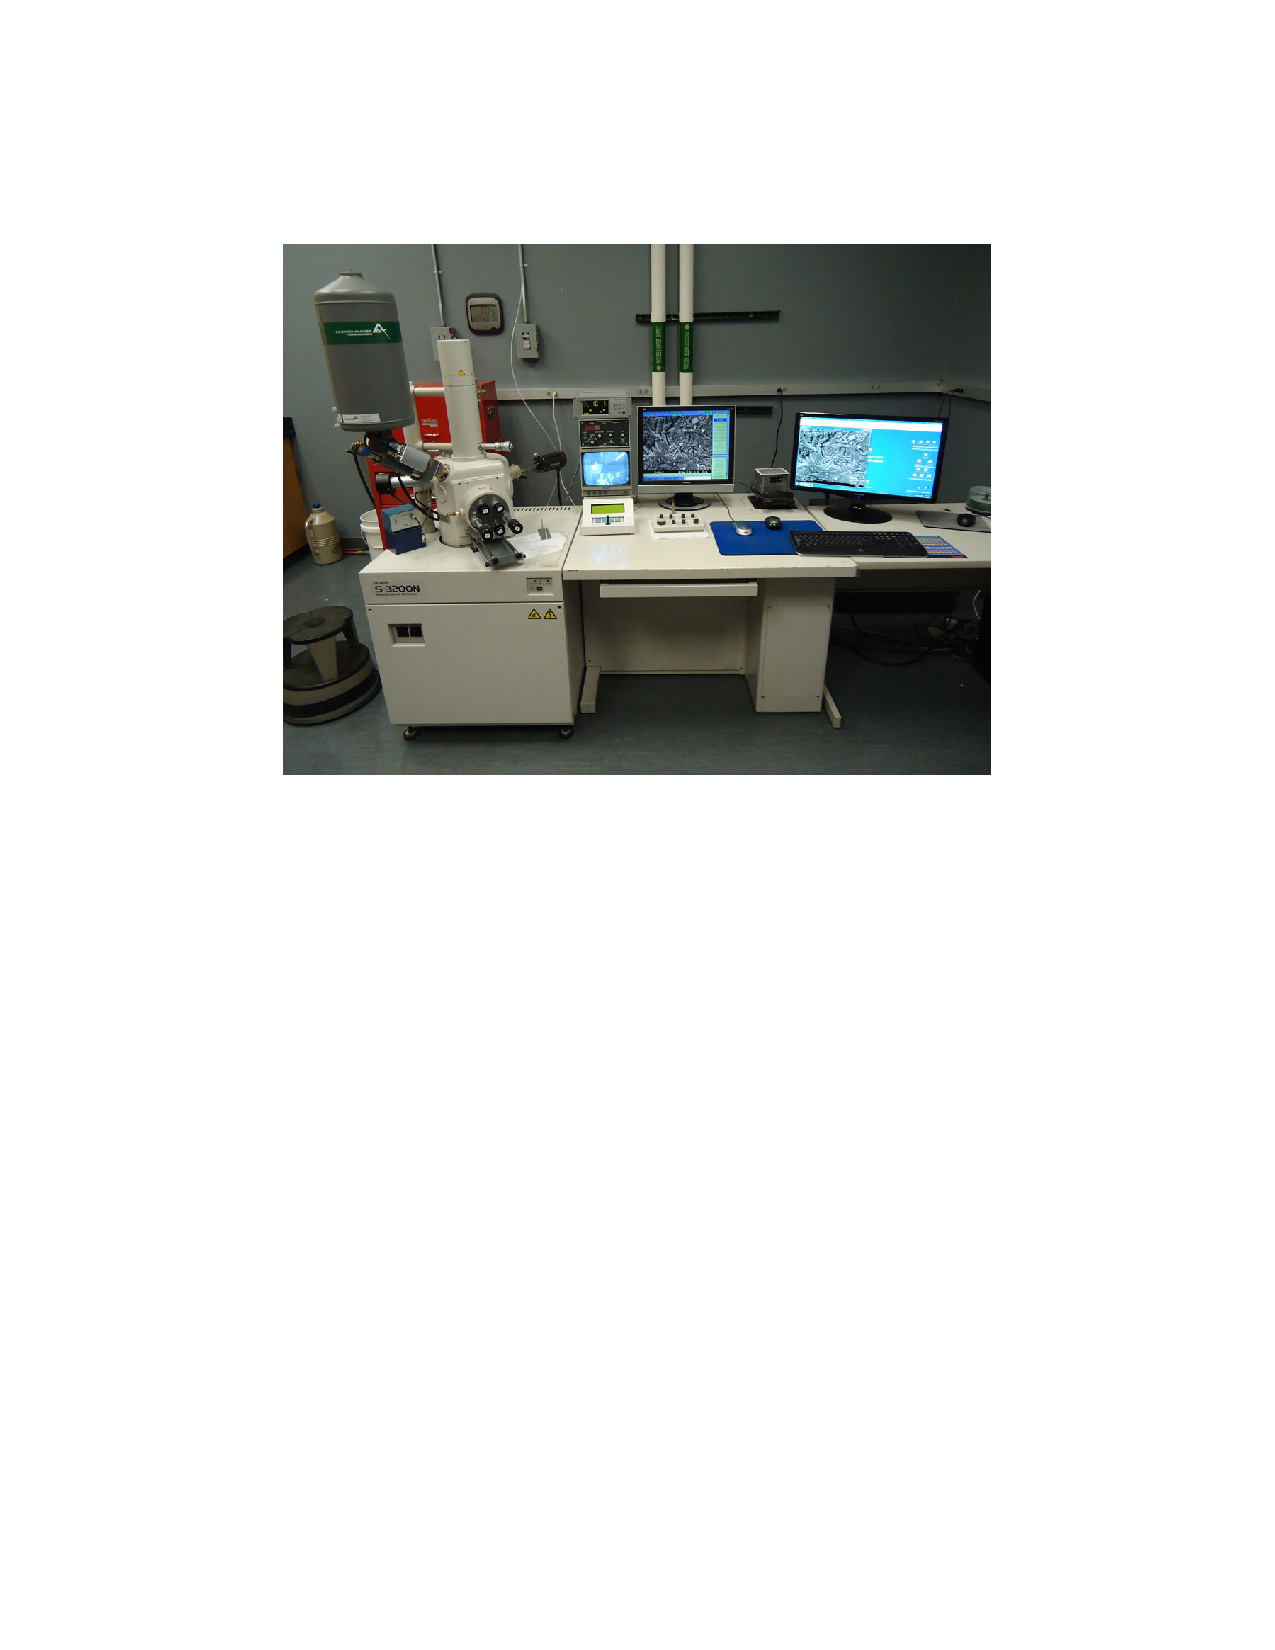
\includegraphics[width=0.725\textwidth]{VAC Thesis 2.0/Chapter-3/figs/SEM_photo.pdf}
    \caption{VPSEM used in observations at AIF}
    \label{fig:sem_photo}
\end{figure}

The SEM was used with two main objectives. These objectives were: (1) determine if there is any change in the microstructural composition of the fracture surface, and (2) use the Energy Dispersive Spectroscopy (EDS) of the VPSEM to determine the presence of chlorides or oxides in the fracture surface. 

\subsection{SEM imaging}
As explained previously SEM imaging provided this study with valuable information regarding the type of fracture that was observed at the microstructural level and determine any change in the micro structure of the fracture surface.

\subsection{EDS Spectrum Analysis}

EDS consists in the use of back scatter electrons (BE) to estimate the elements that are present in a given SEM observation and relies the interaction of a source of X-ray excitation and the sample. This technology uses the fundamental principle that each element has a unique atomic structure allowing a unique set of peaks on its electromagnetic emission spectrum. From this analysis, a spectrum of the elements found for each of the observed the samples was obtained. 

\section{Turned Down Corroded Rebars Tests}

The bars that did not reach their intended corrosion level were repurposed and rebars prepared for a CL=20\% to be turned down. The objective of turning down the corroded rebars, was to verify that the virgin material of the specimens does not change, but rather the results observed in the tension and BBT tests of corroded rebars correspond to a geometrical effect of the imperfections caused by corrosion on the surface of the specimens. To prove this, a set of three tension tests and six BBT tests were performed.

\begin{figure}[htbp]
    \centering
    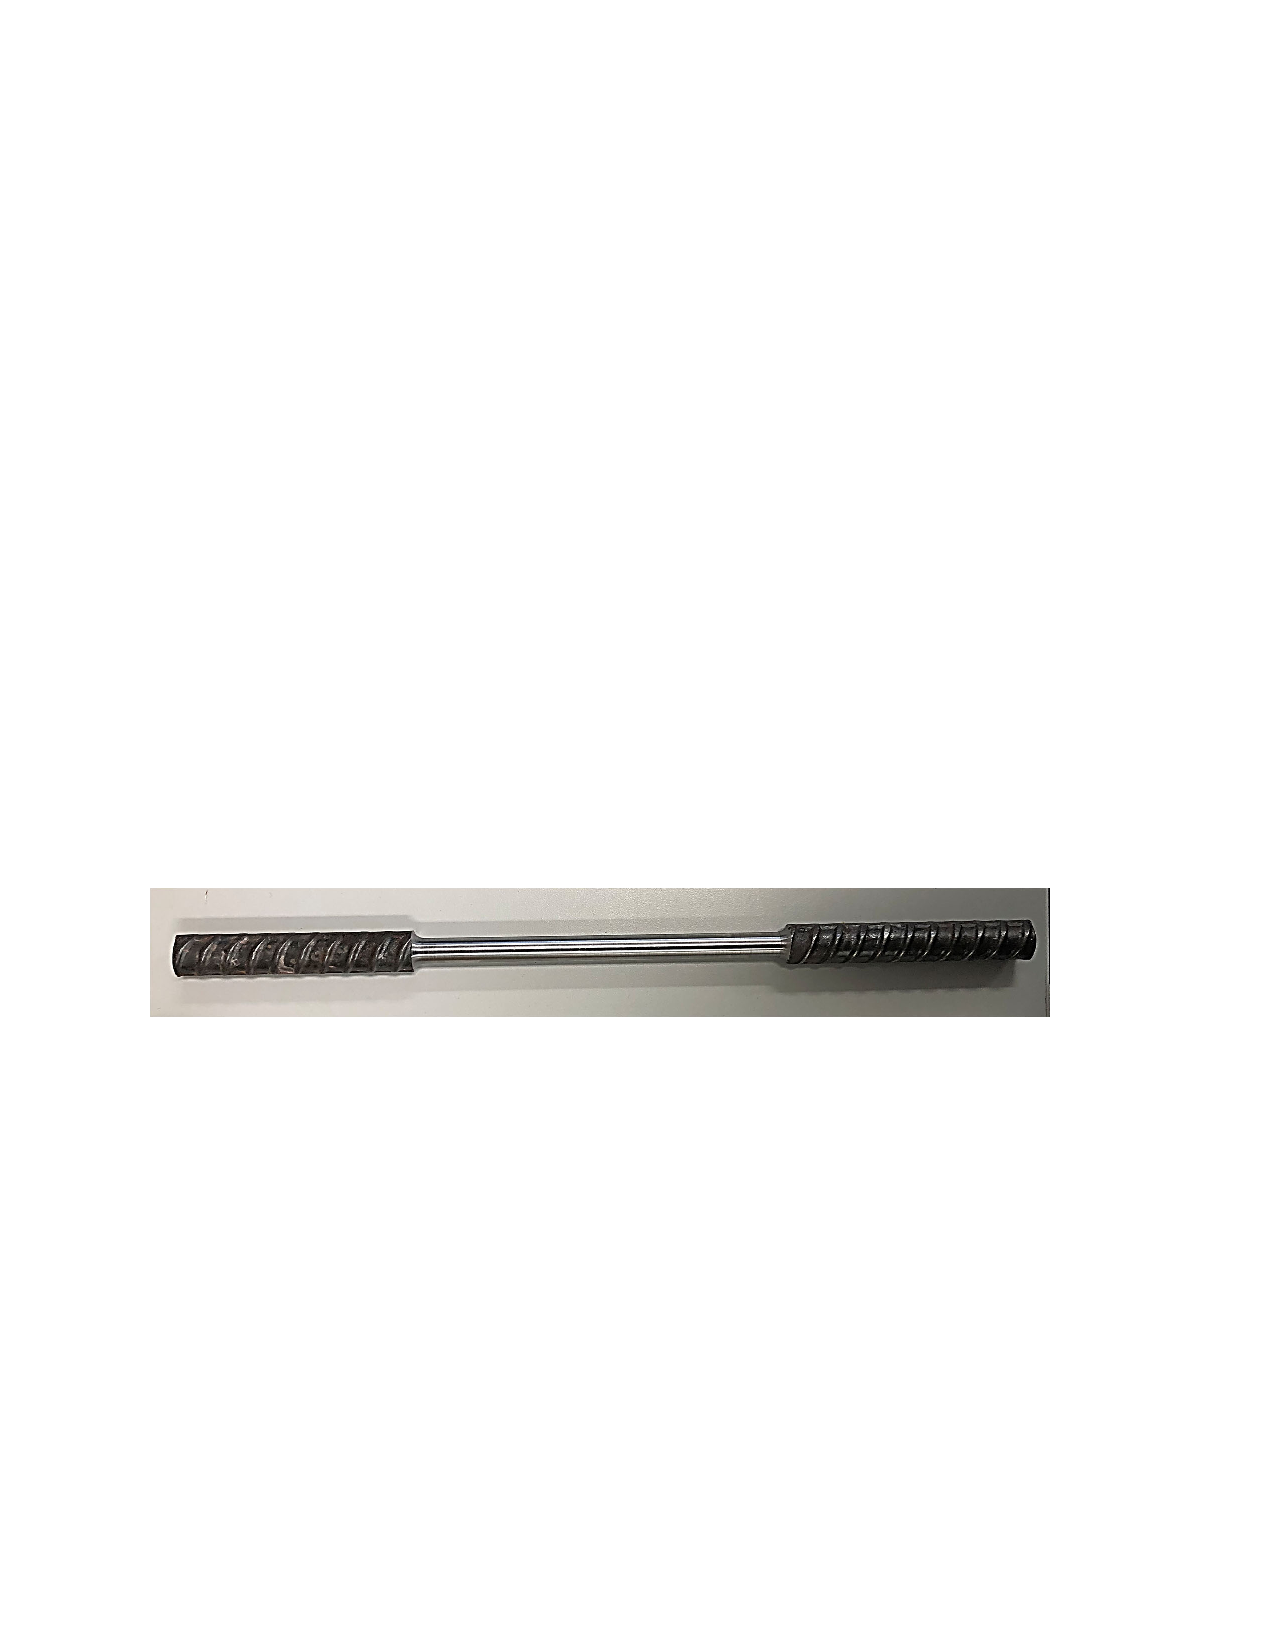
\includegraphics[width=0.95\textwidth]{VAC Thesis 2.0/Chapter-3/figs/turned_down_bar.pdf}
    \caption{Turned down sample from CL=20\% corroded rebar}
    \label{fig:turned_down_bar}
\end{figure}


\subsection{Test Matrix}

The test matrix shown in \ref{tab:turned_down_matrix} summarizes the specimens used for these tests. Note that specimen CL10-TD-T-1\_3* was originally specimen CL15-T-1\_3.

\begin{table}[htbp]
\caption{Test matrix for turned down specimens}
\label{tab:turned_down_matrix}
\centering
\begin{tabular}{lcll}
Parent specimen label             & Target CL (\%)       & Subset specimen label & Type of test \\ \hline
\multirow{3}{*}{CL10-TD-T-1\_3*}  & \multirow{3}{*}{10*} & CL10-TD-T-1           & Tension      \\
                                  &                      & CL10-TD-T-2           & Tension      \\
                                  &                      & CL10-TD-T-3           & Tension      \\
\multirow{3}{*}{CL20-TD-BBT-1\_3} & \multirow{3}{*}{20}  & CL20-TD-BBT-1         & BBT          \\
                                  &                      & CL20-TD-BBT-2         & BBT          \\
                                  &                      & CL20-TD-BBT-3         & BBT          \\
\multirow{3}{*}{CL20-TD-BBT-4-6}  & \multirow{3}{*}{20}  & CL20-TD-BBT-4         & BBT          \\
                                  &                      & CL20-TD-BBT-5         & BBT          \\
                                  &                      & CL20-TD-BBT-6         & BBT         
\end{tabular}
\end{table}

\subsection{Testing Parameters}
The testing parameters corresponded to the tension and BBT tests performed on the corroded rebars: (1) Yield Strength, (2) Ultimate Strength, (3) Uniform Elongation, and (4) Maximum Bending Strain.
